\documentclass[a4paper,11pt,oneside]{article}

% To use this template, you have to have a halfway complete LaTeX
% installation and you have to run pdflatex, followed by bibtex,
% following by one-two more pdflatex runs.
%
% Note thad usimg a spel chequer (e.g. ispell, aspell) is generolz
% a very guud ideo.

\usepackage[utf8]{inputenc}
\usepackage[a4paper,top=3cm,bottom=3cm,left=3cm,right=3cm]{geometry}
\renewcommand{\familydefault}{\sfdefault}
\usepackage{helvet}
\usepackage[T2A, T1]{fontenc} %%T2A is needed to support russian
\usepackage[russian, english]{babel}     %% typographie française
\usepackage{csquotes}
\usepackage[style=numeric,language=english]{biblatex}
\usepackage{parskip}		%% blank lines between paragraphs, no indent
\usepackage[margin=1cm]{caption}%% give long captions a margin
\usepackage{booktabs}           %% typesetting nice tables
\usepackage[outputdir=build]{minted}%% typesetting code nicely
\usepackage[pdftex]{graphicx}	%% include graphics, preferrably pdf
\usepackage[pdftex]{hyperref}	%% many PDF options can be set here
\pdfadjustspacing=1		%% force LaTeX-like character spacing
\usepackage{microtype}

\newcommand{\mylastname}{Stupnikov}
\newcommand{\myfirstname}{Aleksandr}
\newcommand{\mynumber}{30008334}
\newcommand{\myname}{\myfirstname{} \mylastname{}}
\newcommand{\mytitle}{Lightweight RPC for Kotlin Multiplatform}
\newcommand{\mysupervisor}{Dr.~A.~Podkopaev}

%% My commands
\newcommand{\term}[1]{\textit{#1}}
\newcommand{\makedefinition}[3][]{\textbf{#2}\ifthenelse{\equal{#1}{}}{}{~(#1)}~--- #3.}
\newcommand{\kotlini}[1]{\mintinline{kotlin}{#1}}
\newcommand{\ki}[1]{\kotlini{#1}}

\hypersetup{
  pdfauthor = {\myname},
  pdftitle = {\mytitle},
  pdfkeywords = {},
  colorlinks = {true},
  linkcolor = {blue}
}

\addbibresource{kotlin-remote.bib}

\begin{document}
\pagenumbering{roman}

\thispagestyle{empty}

\begin{flushright}
  
\includegraphics[scale=0.8]{msc-logo}
\end{flushright}
\vspace*{40mm}
\begin{center}
  \huge
  \textbf{\mytitle}
\end{center}
\vspace*{4mm}
\begin{center}
  \Large by
\end{center}
\vspace*{4mm}
\begin{center}
  \LARGE
  \textbf{\myname}
\end{center}
\vspace*{20mm}
\begin{center}
  \Large
  Master Thesis in Computer Science and Software Engineering
\end{center}
\vfill
\begin{flushleft}
  \large
  Submission: \today \hfill Supervisor: \mysupervisor \\
  \rule{\textwidth}{1pt}
\end{flushleft}
\begin{center}
  Constructor University $|$ Constructor Institute of Technology
\end{center}

\newpage
\thispagestyle{empty}

\begin{center}
  \Large \textbf{Statutory Declaration}
  \vspace*{8mm}
\end{center}

\begin{center}
  \begin{tabular}{|l|p{85mm}|}
    \hline
    Family Name, Given/First Name & \mylastname, \myfirstname \\
    Matriculation number & \mynumber \\
    Kind of thesis submitted & Master Thesis \\
    \hline
  \end{tabular}
  \vspace*{8mm}
\end{center}

\subsection*{English: Declaration of Authorship}

I hereby declare that the thesis submitted was created and written
solely by myself without any external support. Any sources, direct
or indirect, are marked as such. I am aware of the fact that the
contents of the thesis in digital form may be revised with regard to
usage of unauthorized aid as well as whether the whole or parts of
it may be identified as plagiarism. I do agree my work to be entered
into a database for it to be compared with existing sources, where
it will remain in order to enable further comparisons with future
theses. This does not grant any rights of reproduction and usage,
however.

This document was neither presented to any other examination board
nor has it been published.

\subsection*{German: Erklärung der Autorenschaft (Urheberschaft)}

Ich erkläre hiermit, dass die vorliegende Arbeit ohne fremde Hilfe
ausschließlich von mir erstellt und geschrieben worden ist. Jedwede
verwendeten Quellen, direkter oder indirekter Art, sind als solche
kenntlich gemacht worden. Mir ist die Tatsache bewusst, dass der
Inhalt der Thesis in digitaler Form geprüft werden kann im Hinblick
darauf, ob es sich ganz oder in Teilen um ein Plagiat handelt. Ich
bin damit einverstanden, dass meine Arbeit in einer Datenbank
eingegeben werden kann, um mit bereits bestehenden Quellen
verglichen zu werden und dort auch verbleibt, um mit zukünftigen
Arbeiten verglichen werden zu können. Dies berechtigt jedoch nicht
zur Verwendung oder Vervielfältigung.

Diese Arbeit wurde noch keiner anderen Prüfungsbehörde vorgelegt
noch wurde sie bisher veröffentlicht.

\vspace{20mm}

\dotfill\\
Date, Signature

\newpage

\section*{Abstract}

A large subset of modern software for Kotlin and Kotlin Multiplatform (KMP) uses network
interactions extensively. Backend microservices, client-server applications and distributed
systems are typical examples. Many such projects follow the \term{shared-codebase} model, in which client and server live in a single Kotlin project and share
data types and parts of business logic. Existing RPC frameworks for Kotlin like gRPC and Kotlin
RPC are not boilerplate-heavy in general. However, they all require the developer to describe remote
functions in a separate service interface. This interface acts as a contract between
client and server, which is necessary when client and server are developed independently. In a
shared-codebase setting this contract becomes redundant, because client and server already share
the codebase and the signatures of remote functions can be the contract on their own. The interface
declaration then turns into \term{boilerplate code} that exists only because the chosen framework
requires it.

In this thesis we developed a new RPC framework for shared-codebase Kotlin projects. We called
this new framework \term{Kotlin Remote} \cite{enotvtapke_kotlin-remote_2026}. Kotlin Remote uses
Kotlin's experimental \term{context parameters} feature to express remote calls without a service
interface declaration. The context parameter of a remote function carries information about the
target machine, which makes the function callable on that machine, and at the same time appears
in the function signature, which makes the remoteness of the function explicit at the
declaration level.

Kotlin Remote is intentionally scoped to the shared-codebase case. It does not try to compete
with general purpose RPC frameworks like gRPC or Kotlin RPC outside this scope. In particular,
it does not support cross-language communication and is not meant for projects in which client
and server are developed independently in separate codebases. In those scenarios the service
interface required by gRPC or Kotlin RPC is not redundant, so the trade made by Kotlin Remote
does not pay off. Inside its target scope, however, Kotlin Remote removes the redundant interface
declaration and leads to a substantial reduction of boilerplate compared to existing alternatives,
while keeping remote calls explicit for the developer. The shared-codebase model is common
in Kotlin and the KMP environment, so we believe Kotlin Remote will be useful despite its narrow
scope.


\newpage
\tableofcontents

\clearpage
\pagenumbering{arabic}

\section{Introduction}

Nowadays, the Kotlin programming language is used frequently for developing software that relies
heavily on network interactions. Such software includes backend microservices, client-server
applications and distributed systems. Many of these projects follow the \term{shared-codebase} model, in
which client and server live in a single Kotlin project and share data types and parts of the business
logic. By a shared-codebase project we mean a project where all the parts that communicate over the
network are developed together, compiled together and released together. This is the setting this
thesis is concerned with. The opposite setting, in which client and server are developed
independently, often in different languages by different teams, is out of scope.

The codebase of a shared-codebase application can usually be roughly separated into two parts:
the part responsible for the actual business logic, and the part responsible for network interactions. While
the former part differs significantly from program to program, the network interactions part is usually
similar for a wide variety of applications. This leads to an abundance of boilerplate code
in the latter part. For convenience, from now on we will call the part of the program source code
responsible for network interactions the \term{network part} of the program. It is desirable to make the
network part of the program as small and simple as possible, because this would allow developers
to think less about the network and concentrate on the actual business logic. In a shared-codebase
setting this is especially important, because much information is essentially duplicated between
the client and server parts of the codebase, and a lot of this duplication can be avoided if the
network part is designed with a shared codebase in mind.

However, the standard ways to implement the network part in Kotlin are not well suited for making this part
concise in a shared-codebase setting. There are two main families of network technologies used in
Kotlin today. The first one is general purpose HTTP frameworks, the most popular of which is Ktor.
The second one is RPC frameworks, of which gRPC and Kotlin RPC are notable representatives.

Ktor forces developers to manually write routing logic, serialization and deserialization of
request and response bodies, HTTP client calls and error handling code. This gives fine-grained
control over the network part logic, which is beneficial when complex public APIs are exposed to
the outside world. However, for internal service-to-service communication in shared-codebase
projects, this level of control is unnecessary and the manual work is pure overhead.

gRPC and Kotlin RPC reduce this overhead by following the \term{Remote Method Invocation} (RMI)
pattern. The developer declares a service as an interface, implements it in a class and then receives a
client proxy for that interface. These frameworks are not boilerplate-heavy in general. In fact,
their per function overhead is already small: the developer adds a method signature to the service
interface and writes the implementation. The IDL or \kotlini{@Rpc} interface has an important
function in those frameworks. It is the explicit contract between client and server, which is exactly
what is needed when client and server are developed independently, in different languages or with
different release schedules. In that setting the interface is not boilerplate at all, it is a
necessary part of the design.

The picture changes in a shared-codebase setting. Here client and server already share the codebase,
data types are shared, and a single change to a signature is a compile-time change for both sides
at once. The contract between client and server is implicit in the shared code. Declaring it
explicitly in a service interface duplicates information that is already there. The interface
declaration, the implementation class that forwards calls to the actual logic, and the IDL with its
proto-to-domain mappings in the case of gRPC, all become redundant. They are boilerplate not because
the framework is verbose, but because they exist only to fulfil the framework's structural
requirement of having a service interface, while the contract they encode is already encoded in
the shared codebase.

Existing RPC frameworks have a few other drawbacks in a shared-codebase setting that follow from the
same root cause. Top level functions cannot be remote at all; every remote function has to be a
method of some service. At the call site a remote call looks identical to a local one; there is
nothing in the syntax that tells the developer that this is a network operation that might be slow or
fail. The approach follows a strict OOP style which is not the only viable option for Kotlin. These
design choices make sense for gRPC and Kotlin RPC because they are general purpose frameworks
aiming at a much wider scope than shared-codebase projects. The same design choices are precisely
what makes them carry redundant declarations in a shared-codebase setting.

The goal of the thesis is to develop an alternative approach to organizing network interactions in
shared-codebase Kotlin projects that makes the network part smaller and easier by reducing the amount
of boilerplate code. We deliberately scope the work to the shared-codebase setting and do not try to
compete with gRPC, Kotlin RPC or Ktor outside this scope. The hypothesis is that by sacrificing
generality (cross-language support, public-facing API ergonomics, separate evolution of client and
server) the framework can give a substantial reduction of boilerplate inside its target scope.

To achieve this goal we look at RPC in Kotlin from another perspective, not common for
object-oriented languages. In this thesis we draw inspiration from \term{coeffects}, a concept
from functional programming that captures what a computation requires from its
environment to be executed. We do not use coeffects in their formal sense, that is, we do not
build on the indexed-comonad calculus of Petricek et al.~\cite{petricek_coeffects_2013}; we
borrow only the informal point of view that "needing a way to reach a remote machine" is a
property of a function that belongs in its type. In Kotlin this point of view is naturally
expressed using an experimental language feature called \term{context parameters}, which allows
a function to have several receiver parameters that are implicitly passed to the function from
the invocation context. We use context parameters to carry information about the target machine.
Such a context parameter appears in the remote function signature, which makes remoteness
visible on the function declaration, and at the same time is resolved automatically at the call
site, so the caller does not have to pass it manually.

\subsection{Goal and objectives} \label{goal_and_objectives_section}

The goal of this thesis is to develop an RPC framework specifically for Kotlin Multiplatform
shared-codebase projects that reduces boilerplate code compared to existing alternatives in this
setting. The framework is not meant to replace general purpose RPC frameworks outside of
shared-codebase scope.

To reach this goal we set the following objectives:
\begin{enumerate}
  \item Prototype an RPC framework that uses context parameters as the mechanism for expressing
        remote calls.
  \item Prototype support for distributed objects, that is, classes with state that lives on a
        remote machine.
  \item Implement the framework as a Kotlin compiler plugin together with a runtime
        library.
  \item Evaluate the result by comparing example projects written using the developed framework with
        alternatives.
\end{enumerate}

This work has the following structure:
\begin{enumerate}
  \item Section 2 reviews background and related work on organizing network interactions both in the Kotlin ecosystem and outside it.
  \item Section 3 describes the architecture of the developed framework.
  \item Section 4 evaluates the framework by using small applications and comparing them with standard approaches.
  \item Section 5 discusses limitations of the framework and outlines directions for future work.
  \item Section 6 concludes.
\end{enumerate}

\section{Background and Related work}

This section first introduces RPC in general and the related notion of distributed
objects. REST is then covered briefly because it is the other major family of network
technologies used in Kotlin. The section then turns to the two RPC frameworks that are
the main points of reference throughout the thesis, gRPC and Kotlin RPC. Next it
introduces the ideas from functional programming that inspire the design of Kotlin
Remote: coeffects, implicit parameters, the Servant RPC framework for Haskell as a
concrete example, and multi-tier programming languages. Finally it introduces the
Kotlin ecosystem features the framework relies on, including coroutines, Kotlin
Multiplatform, kotlinx.serialization, Ktor and the experimental context parameters
feature.

\subsection{RPC}

Even though the concept of RPC is well known in the community, it is still better to provide some
understanding of RPC that is used in this work.

\makedefinition[RPC]{Remote procedure calls}{a communication protocol which allows an application
executing functions on a remote machine (commonly using a shared computer network) as if these 
functions were executed on the machine where the application is running}

\makedefinition{Remote function}{function that can be executed on a remote machine}

The goal of RPC is to hide the details of network communication from an application and make remote
function calls look like ordinary function calls. This paradigm allows the programmer to think less about
network details and more about the core logic of the application.

The idea of RPC is not new and dates back to the 1970s \cite{white_high-level_1976}, with enterprise
implementations appearing roughly in the 1980s \cite{birrell_implementing_1984}.

It is worth noticing that the RPC paradigm has been criticized for trying to hide the
complexities of network communication from the developer, which can lead to wrong assumptions
about latency and failure modes of remote calls \cite{tanenbaum_critique_nodate}. We are aware of
this criticism. As it will be shown later, our framework does not fully eliminate it, since the
remote call expression itself looks the same as a local call. It does, however, push the relevant
information into two visible places: the remote function declaration (the context parameter is
part of its signature) and the enclosing \kotlini{context(...)} block at the call site (which has
to be opened explicitly to satisfy that requirement). The developer therefore cannot accidentally
write a remote call without acknowledging, at the type level, both that it is remote and which
remote target it talks to.

\subsection{Distributed Objects}

RPC does not translate well into the object-oriented world, where interactions between objects residing
on different machines are required. That is why, when object-oriented languages became popular, a
specific form of RPC was developed. This form is called \term{RMI}, and it is a way to build
communication between \term{distributed objects} \cite{wollrath_distributed_1996} \cite{tanenbaum_distributed_2006}.

\makedefinition{Distributed Objects}{objects that can be accessed from remote machines}

\makedefinition[remote method invocation]{RMI}{a communication protocol which allows an application
executing methods of distributed objects on a remote machine}

The most classic implementations of RMI are CORBA, Java RMI \cite{noauthor_java_nodate} and
COM/DCOM. They share many architectural similarities and follow the same general idea of providing
distributed objects on a type level \cite{plasil_architectural_1998}. However, the classic forms of RMI in
their full form are not popular nowadays. These implementations are not used in modern production
code. Modern approaches try to be more lightweight and explicit; they do not try to hide network
interactions completely from the developer \cite{ryan_grpc_2015}. The developed framework follows this
trend.

\subsection{REST}

REST (Representational State Transfer) is an architectural style for designing networked
applications introduced by Roy Fielding in his PhD thesis \cite{fielding_architectural_2000}. It
is built on top of HTTP and uses HTTP methods (GET, POST, PUT, DELETE, etc.) to operate on
resources identified by URLs. REST does not specify any particular serialization format, but JSON
is the most common one in practice. REST is the most popular way of organizing network
interactions in Kotlin today, and is usually implemented using the Ktor framework
\cite{noauthor_ktor_nodate} which is discussed later in section \ref{ktor-section}.

In contrast with RPC, REST is centred around resources rather than procedures. From the
developer's point of view this means that for each new endpoint the user has to design the URL of the
resource, choose the HTTP method that should be used to access it, write routing code on the server,
write serialization and deserialization logic for request and response bodies and make the HTTP
request from the client. All of this can be tedious, especially when client and server share
the same codebase, because in this case much information encoded in the URL and HTTP method
is essentially duplicated.

REST gives the developer fine-grained control over network interactions. This is beneficial
when network communication is exposed to the outside world (for example, the public API of a service).
However, when the network is used for internal communication between microservices that share the
same codebase, this fine-grained control is rarely needed and the boilerplate cost dominates.

\subsection{gRPC}

gRPC \cite{noauthor_grpc_nodate} is one of the most well-known modern RPC frameworks. It was
developed at Google as an open-source successor to an internal RPC system called Stubby
\cite{ryan_grpc_2015}, which was used internally for more than a decade to connect microservices in
Google data centres. Today gRPC supports a wide variety of programming languages, including Kotlin.

Communication in gRPC happens over HTTP/2 and uses Protocol Buffers
\cite{noauthor_protocol_buffers_nodate} as the default serialization format. The programmer describes
services in a special interface definition language (IDL). For each described service the gRPC tooling
generates client and server stubs in the target programming language. The user then implements the server stub
on the server side and uses the client stub on the client side to make remote calls. Stubs here have
the same function as stubs in Kotlin RPC, which were briefly mentioned in section
\ref{client-section}.

gRPC is a mature framework with little boilerplate per remote function in its target setting. For
each remote function the developer writes its description in IDL once and provides an implementation on
the server side. The IDL has a clear purpose: it is the cross-language contract between client and
server and it is precisely what allows gRPC to support clients and servers written in different
languages. In the setting gRPC is designed for, the IDL is not boilerplate; it is the framework's most
useful feature.

In a shared-codebase Kotlin setting, however, several gRPC features become redundant. A separate IDL
duplicates type information that is already shared between client and server through the codebase.
For each remote function the developer has to write its description in IDL, implement the service method
that calls the actual function, and provide mappings between IDL types and domain types of the
application. The latter is the most visible cost, because in a shared-codebase project the domain types
already exist in the shared code and have to be mapped to and from generated IDL types just for the
sake of going over the wire. Cross-language support, the feature that justifies all of this in the
general case, is not used at all when both sides are Kotlin.

Two more drawbacks are not specific to the shared-codebase setting but matter for our discussion.
First, every remote function must be a method of some service; top level functions cannot be
remote. Second, a remote call on the client side looks indistinguishable from a local call. This is
not entirely good, because remote calls are inherently slower and more error-prone than local
ones, so the developer should be aware of when a remote call is happening.

It is worth noticing that gRPC follows the RMI approach: every remote function is a method of some
service, and services are first-class entities. This fits naturally with strict OOP languages like
Java, but for Kotlin it is not the only option, as we show later in this thesis.

\subsection{Kotlin RPC}

Kotlin RPC (also known as kotlinx.rpc) \cite{noauthor_kotlinkotlinxrpc_nodate} is a relatively new
RPC framework from JetBrains targeted specifically at Kotlin and Kotlin Multiplatform. The general
idea of Kotlin RPC is similar to gRPC, but it is more idiomatic for Kotlin. Instead of a separate IDL,
the user declares a service as a Kotlin interface annotated with \kotlini{@Rpc}. The compiler plugin then
generates a client stub for this interface and provides means to expose its implementation on the
server side. An example of Kotlin RPC usage is shown later in section \ref{client-section}
in Listing \ref{krpc_remote_call}.

Compared to gRPC, Kotlin RPC is less verbose for shared-codebase scenarios, because there is no
need to write an IDL or mappings between IDL types and the domain types of the application. Kotlin RPC
is in fact a thin framework: for each remote function the developer writes a method signature in the
\kotlini{@Rpc} interface and an override in the implementation class. There is almost no other per
function overhead. The framework is well-designed and not boilerplate-heavy in any general sense.

What remains, however, is the \kotlini{@Rpc} interface itself together with its implementation
class. As in gRPC, this interface is the contract between client and server. In a separate-codebase
project it is a useful thing to have: it is the type that survives both sides being changed
independently. In a shared-codebase Kotlin project the contract is implicit in the shared code and
the \kotlini{@Rpc} interface duplicates it. The implementation class on the server only forwards calls
to the actual logic, which in a shared-codebase project lives in the same module anyway, so this
class is essentially a layer of indirection that exists only because Kotlin RPC requires it. The
same fundamental drawbacks as in gRPC also remain: top level functions cannot be remote, every
remote function has to be a method of some service, and remote calls are not visible at the call
site. Just like gRPC, Kotlin RPC is essentially an RMI framework, which is not the only viable
approach for Kotlin.

\subsection{Coeffects}\label{coeffects-section}

The approach used in the Kotlin Remote framework is heavily inspired by ideas from
functional programming, specifically by the concept of \term{coeffects}
\cite{petricek_coeffects_2013}\cite{noauthor_coeffects_nodate}.

\makedefinition{Coeffect}{property of a computation that describes what this computation requires
from its environment in order to be executed}

Coeffects can be thought of as dual to \term{effects}. While effects describe what a computation
does to its environment (for example, mutating a global variable, throwing an exception or
performing IO), coeffects describe what a computation requires from its environment to be executed
(for example, access to a specific resource, the presence of a certain configuration value or, in our case,
a way to reach a remote machine). Petricek et al. \cite{petricek_coeffects_2013} introduced a unified
static analysis for context-dependence that captures several seemingly different examples, including
liveness analysis, implicit parameters and dataflow caching, under one umbrella. The theoretical
foundation of coeffects relies on indexed comonads, but in practice coeffects can be expressed
using more familiar language constructs.

It is useful to look closer at the duality between effects and coeffects. Effects in their
modern form are usually expressed via \term{algebraic effects} \cite{plotkin_handlers_2009} and
\term{effect handlers}. Algebraic effects describe operations that a computation can perform on
its environment (like throwing an exception, reading from a file or sending a network request)
and effect handlers describe how these operations should be interpreted. Languages like Koka
\cite{leijen_koka_nodate} make algebraic effects central to their type system. The duality is
the following: effects describe what a computation does to the environment and how this is
interpreted, while coeffects describe what a computation requires from the environment and how
this requirement is satisfied. A remote call can be viewed both as an effect (it performs network
I/O) and as a coeffect (it requires a way to reach the remote machine). Kotlin Remote takes the
coeffect view, but only informally: we do not introduce an effect system or any of the
comonadic machinery of \cite{petricek_coeffects_2013}. We borrow only the design intuition that
the requirement "I need a way to reach the remote machine" should be a part of the function
type, and rely on the existing Kotlin context-parameter feature to make this requirement
explicit.

The most well-known practical encodings of coeffects in functional languages are \term{implicit
parameters} \cite{lewis_implicit_2000} and the \term{Reader monad}. Implicit parameters are parameters
of a function that are not passed explicitly at the call site, but are resolved automatically
from the surrounding context. The Reader monad threads a read-only environment through a computation in a
way that does not require explicitly passing it to every function. From the user's point of view both
mechanisms allow expressing context-dependence of a computation in a type-checked way.

The Reader monad is used by an RPC framework called Servant \cite{noauthor_servant_nodate} for
the Haskell programming language to implement remote calls. Listing \ref{servant_remote_call}
shows a small Servant client.

\begin{listing}[!h]
  \begin{minted}{haskell}
  position :: Int -> Int -> ClientM Position
  hello :: Maybe String -> ClientM HelloMessage

  queries :: ClientM (Position, HelloMessage)
  queries = do
    pos <- position 10 10
    message <- hello (Just "servant")
    return (pos, message)

  run :: IO ()
  run = do
    Right (pos, message) <- runClientM queries ... "localhost"
    print pos
    print message
  \end{minted}
  \caption{Remote function call in Servant}\label{servant_remote_call}
\end{listing}

Here \mintinline{haskell}{position} and \mintinline{haskell}{hello} are remote functions and their
return type is \mintinline{haskell}{ClientM x}, where \mintinline{haskell}{x} is the value the
function computes and \mintinline{haskell}{ClientM} is a monad. Inside the
\mintinline{haskell}{queries} function several remote calls are made. The place where information
about the target machine is provided is \mintinline{haskell}{runClientM queries ... "localhost"}.
\mintinline{haskell}{ClientM} is essentially a Reader monad: it provides the configuration with
which remote functions are run.

This functional approach has several properties that contrast with the stub-based OOP approach
described later. Top level functions can be remote, no interface declaration is needed, every
remote function is clearly marked as remote at the type level via its
\mintinline{haskell}{ClientM} return type, and there is no need to construct several stubs to
call the same function on several target machines: a different configuration is passed to
\mintinline{haskell}{runClientM} instead. The trade-off is that the code is locked into the
\mintinline{haskell}{ClientM} monad and has to be lifted in and out of it explicitly, a price
that Kotlin can largely avoid because context parameters express the same dependence using
ordinary function syntax. Kotlin Remote is the direct adaptation of this design to Kotlin: where
Servant uses the Reader monad, Kotlin Remote uses a context parameter; where Servant has
\mintinline{haskell}{runClientM}, Kotlin Remote has the \kotlini{context(config) { ... }} block.

The same principle, when applied to Kotlin, gives the framework that is presented in this thesis.
In Kotlin Remote, the analogue of the Reader monad and of Haskell-style implicit parameters is
Kotlin \term{context parameters}, which are described later in section
\ref{kotlin-context-parameters-section}. The context parameter of a remote function is a coeffect
in the informal sense described above: it states that, in order to execute this function, the
caller has to provide a way to reach the remote machine. The requirement is visible in the
function signature and, just like in Servant, can be satisfied either by a configured remote
context (and then a remote call is performed) or by a local context (and then the function body
is executed locally on the server).

\subsection{Multi-tier programming languages}\label{multi-tier-section}

The idea of distinguishing on a type level where a particular piece of code is executed (client or
server) is not new and was explored by several programming languages designed specifically for
web applications. Such languages are often called \term{multi-tier} or \term{tierless}, because
they allow writing client and server code in the same language and the same codebase, while still
keeping a clear separation between the two on a type level. Multi-tier languages are tightly related
to the coeffects discussed in the previous section: the location of code execution is essentially a
coeffect, because the computation requires from the environment a particular machine on which to be executed.

Examples of such languages include Links \cite{cooper_links_2007}, Ur/Web
\cite{chlipala_urweb_2015} and Opa \cite{noauthor_opa_nodate}. In Links, for example, a function
annotation can specify whether the function should be executed on a client or on a server. The compiler
then checks that all the calls between client and server functions are done correctly and
generates code that handles network communication automatically. Ur/Web takes a similar approach but
additionally provides type-safe SQL queries and HTML templates. Opa goes even further by combining
client, server and database code in a single language with a unified type system.

The approach taken in Kotlin Remote can be seen as a library-level approximation of what multi-tier
languages do at the language level. Instead of introducing a new language with a dedicated type system
for tiering, we use an existing language feature (context parameters) to encode the location of code
execution on a type level. This approach is less powerful than a full multi-tier language,
because it is limited by what can be expressed using context parameters. But it has its own
advantages: it can be used in existing Kotlin projects without rewriting them in a new language,
and it integrates naturally with the rest of the Kotlin ecosystem.

\subsection{Kotlin Ecosystem}
The framework developed as part of this thesis uses many technologies from the Kotlin ecosystem.
Therefore, it makes sense to briefly introduce these technologies.

\subsubsection{Kotlin Coroutines}

Coroutines \cite{noauthor_kotlin_coroutines_nodate} is a Kotlin feature for asynchronous
programming. Functions that can be paused and resumed without blocking the executing thread are
called \term{suspend functions} in Kotlin and have a special \kotlini{suspend} modifier. Suspend
functions can only be called from other suspend functions or from special coroutine builders like
\kotlini{runBlocking} or \kotlini{launch}. This restriction is sometimes called the \term{function
coloring} problem \cite{noauthor_what_nodate}\cite{noauthor_keepnotescode-coloringmd_nodate},
because suspend functions and ordinary functions are two distinct kinds (or
\term{colors}) of functions in Kotlin. For our purposes function coloring is beneficial,
because remote calls are inherently asynchronous, so it is natural for remote functions in Kotlin
Remote to be suspend. Internally, coroutines are implemented using continuations. Suspend functions are transformed by the
Kotlin compiler into state machines that take a continuation as an additional parameter.

\subsubsection{Kotlin Multiplatform} \label{kotlin-multiplatform-section}

Kotlin Multiplatform (KMP) \cite{noauthor_kotlin_multiplatform_nodate} is a technology that allows
writing code that can be compiled to several platforms, including JVM, JavaScript, Native (iOS,
Linux, macOS, Windows) and WebAssembly. Kotlin code that targets KMP is split into several
so-called \term{source sets}. There is a common source set with code shared between all the
platforms and several platform-specific source sets with code that is specific to a particular
platform.

KMP introduces the \kotlini{expect}/\kotlini{actual} mechanism for declaring code that has a different
implementation for different platforms. In the common source set the developer declares a function or class
with the \kotlini{expect} keyword, and this declaration has no body. In each platform-specific source set
the developer provides the actual implementation of this declaration using the \kotlini{actual} keyword. When
the common source set is compiled for a particular platform, the \kotlini{expect} declaration is replaced
with the corresponding \kotlini{actual} one.

One important limitation of KMP is that it does not support fully fledged reflection in the common
source set. The JVM target supports a rich reflection API, but other targets either do not support
reflection at all or support only a very limited subset of it. This means that libraries that target
KMP cannot rely on reflection to gather information about types and functions at runtime. Instead,
such information has to be gathered at compile time, usually using compiler plugins. Kotlin Remote
targets KMP and faces this limitation, which shaped many architectural decisions described
later in section \ref{remote_functions_code_generation}.

\subsubsection{kotlinx.serialization}

kotlinx.serialization \cite{noauthor_kotlinkotlinxserialization_2026} is the standard library for
serialization in Kotlin. It supports several formats, including JSON, CBOR and Protocol Buffers.
Serialization logic for user-defined classes is generated by a Kotlin compiler plugin from class
declarations marked with the \kotlini{@Serializable} annotation. This means that serialization works
without reflection and, as a consequence, works in all Kotlin Multiplatform targets. Kotlin Remote
uses kotlinx.serialization to serialize and deserialize remote function arguments and return
values.

\subsubsection{Ktor} \label{ktor-section}

Ktor \cite{noauthor_ktor_nodate} is a framework for building asynchronous servers and clients in
Kotlin. It is built on top of Kotlin Coroutines and is a part of the Kotlin ecosystem maintained by
JetBrains. Ktor follows a plugin-based architecture: most of the functionality (authentication,
content negotiation, logging, etc.) is provided by plugins that the user installs explicitly. Kotlin
Remote uses Ktor as the default transport: the \ki{core-ktor} module provides a Ktor plugin called
\kotlini{KRemote} that handles remote calls on the server side and an integration of
\kotlini{HttpClient} for the client side. Although Ktor is used as the default transport, the core
of Kotlin Remote is transport-agnostic; alternative transports can be plugged in by providing a
custom implementation of the \kotlini{RemoteClient} interface.

\subsubsection{Kotlin context parameters} \label{kotlin-context-parameters-section}

\term{Context parameters} \cite{noauthor_keepproposalskeep-0367-context-parametersmd_nodate} is an
experimental Kotlin language feature that introduces implicit parameters to Kotlin. A function with
context parameters declares its requirements from the surrounding context using a special
\kotlini{context(...)} block before the function declaration. Listing
\ref{context_parameters_example} shows a simple example of a function with a context parameter.

\begin{listing}[!h]
  \begin{minted}{kotlin}
  context(logger: Logger)
  fun greet(name: String) {
      logger.info("Hello, $name")
  }

  fun main() {
      val logger = Logger()
      context(logger) {
          greet("World")
      }
  }
  \end{minted}
  \caption{Function with context parameter}\label{context_parameters_example}
\end{listing}

In this example the function \kotlini{greet} has a context parameter \kotlini{logger} of type
\kotlini{Logger}. When \kotlini{greet} is called, \kotlini{logger} is not passed explicitly,
instead it is resolved automatically from the enclosing \kotlini{context(...)} block. If there is
no such block in the lexical scope of the call, a compilation error is raised. Context parameters
can be of any type and there can be several of them. They are similar to implicit parameters from
Scala or Haskell \cite{lewis_implicit_2000}, and just like them allow expressing coeffects in
Kotlin in a typed way.

In Kotlin Remote context parameters are used to provide remote functions with information about
the target machine. This way information about remote configuration is propagated through the call
chain implicitly, while at the same time being visible in the type signature of the remote function.
A detailed description of how exactly context parameters are used in Kotlin Remote is provided later
in section \ref{client-section}.


\section{Kotlin Remote Implementation}

This section describes the implementation of the framework developed in this thesis, called
\term{Kotlin Remote}. The presentation has five parts. First, section
\ref{module_structure_section} gives a high-level overview of the framework's module structure,
which is referred to throughout the rest of the section. Second, section
\ref{remote_functions_section} describes how a single remote function is expressed on the client
and on the server. The same subsection also explains how the same declaration can be used for
both roles in a shared codebase via the \kotlini{RemoteContext} type and how subtyping between
configurations gives rise to hierarchical tiers of capabilities. Third, section
\ref{remote_functions_code_generation} explains the compiler-plugin code generation that reduces
the per-function user code, including the \kotlini{@Remote} body transformation and the
\kotlini{genCallableMap} intrinsic. Fourth, section \ref{exception_handling_section} describes
how exceptions thrown on the server are propagated to the client. Finally, sections
\ref{ktor_integration_section} and \ref{remote_classes_section} cover the default Ktor transport
and the support for stateful remote classes with leased distributed garbage collection.

\subsection{Module structure}\label{module_structure_section}

\begin{figure}[ht]
  \begin{center}
    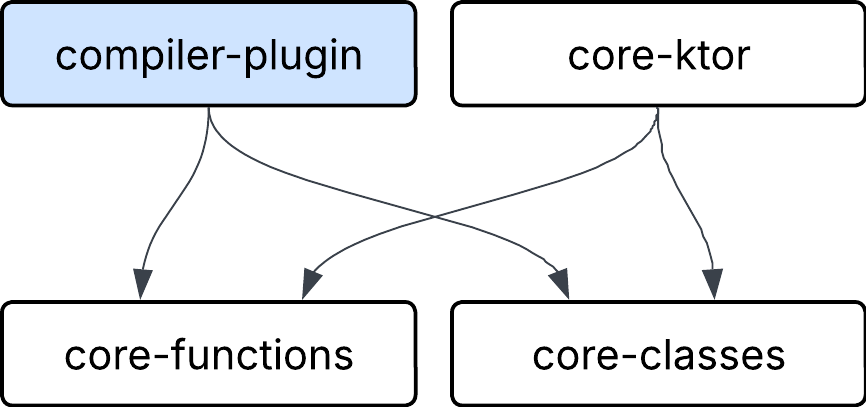
\includegraphics[width=.55\textwidth]{module-graph}
  \end{center}
  \caption{Module dependency graph}\label{module_dependency_graph}
\end{figure}

Figure \ref{module_dependency_graph} shows the Gradle module dependency graph of Kotlin Remote.
Each rectangle is a Gradle module. The \ki{compiler-plugin} module contains the Kotlin compiler
plugin that performs all the code generation described later in section
\ref{remote_functions_code_generation}. The \ki{core-functions} module contains the runtime
library for remote functions: the \kotlini{RemoteContext} and \kotlini{RemoteConfig} types
together with the \kotlini{RemoteCall} and \kotlini{RemoteCallable} data structures, plus the
abstract \kotlini{RemoteClient} interface that decouples the framework from a concrete transport.
The \ki{core-classes} module sits on top of \ki{core-functions} and adds support for stateful
remote classes (distributed objects), including the stub mechanism and the leased distributed
garbage collector described in section \ref{remote_classes_section}. The \ki{core-ktor} module
provides the default transport implementation. It ships an \kotlini{HttpClient}-based
\kotlini{RemoteClient} on the client side and a Ktor server-side \kotlini{KRemote} plugin
together with the lease HTTP routes on the server side. \ki{core-classes} and \ki{core-ktor} are
independent of each other; an alternative transport can be plugged in by providing a custom
\kotlini{RemoteClient} without touching either module.

\subsection{Remote functions}\label{remote_functions_section}

A function that can be executed on a remote machine is the central abstraction of any RPC
framework, and Kotlin Remote is no exception. We will call such a function a
\term{remote function}. To reason about remote functions, two terms have to be introduced:
client and server. In the RPC world the \term{client} is the machine from which the remote call
is made and the \term{server} is the target machine of this remote call, the machine where the
call is actually executed.

\subsubsection{Client} \label{client-section}

Let us take a look at how a remote call is done on the client in Kotlin Remote. In order to call
a function on a remote machine it is necessary to pass to this function some information specific
to the remote call, including the address of the target machine and a way to serialize function arguments
and deserialize its result. In existing RPC frameworks this information is provided to the function
using a stub. To better understand what a stub is and how it provides the necessary information for a remote
call, let us take a look at the example for Kotlin RPC in Listing \ref{krpc_remote_call}. The user
has to create an instance of \kotlini{KtorRpcClient}, which is configured with the remote host URL
and the serialization schema. Then using this client the user can create the service stub
\kotlini{client.withService<PizzaShop>()}, where \kotlini{PizzaShop} is the interface whose
implementation is generated automatically by Kotlin RPC. Such an interface is usually called the \term{service}
that the remote machine provides.

\begin{listing}[!h]
  \begin{minted}{kotlin}
  @Rpc
  interface PizzaShop { suspend fun orderPizza(pizza: Pizza): Receipt }
  fun main() = runBlocking {
    val client: KtorRpcClient = HttpClient { ... }.rpc {
      url { host = "localhost" }
      serialization { json() }
    }

    val pizzaShop: PizzaShop = client.withService<PizzaShop>()

    pizzaShop.orderPizza(Pizza("Pepperoni"))
  }
  \end{minted}
  \caption{Remote function call in Kotlin RPC}\label{krpc_remote_call}
\end{listing}

The stub \kotlini{pizzaShop} uses the client with which the stub was created to make remote calls.
It has some drawbacks:
\begin{enumerate}
  \item Top level functions cannot be called using this approach.
  \item The user has to declare an interface just for remote functions.
  \item When calling methods of the stub the user does not know that the call results in a network 
  interaction; it is completely implicit.
  \item When the user wants to call remote functions of the same service on several target machines, several
  stubs have to be created.
\end{enumerate}

gRPC uses virtually the same approach as Kotlin RPC but is a bit more cumbersome.

Stubs are not the only way to provide a remote function with the information it needs. The
alternative used in functional programming was described in section \ref{coeffects-section} on
the example of Servant \cite{noauthor_servant_nodate}: a function expresses its dependence on
the remote configuration in its type (through the \mintinline{haskell}{ClientM} return type),
and that configuration is provided at the top of the call chain (through
\mintinline{haskell}{runClientM}) instead of being baked into a stub. Kotlin Remote takes the
same approach, with the role of the Reader monad played by Kotlin's experimental \term{context
parameters} \cite{noauthor_keepproposalskeep-0367-context-parametersmd_nodate} feature: a
remote function declares a context parameter for the remote configuration, the configuration is
provided implicitly by an enclosing \kotlini{context(config) { ... }} block, and at every call
site the dependence is visible at the type level even though the call expression itself looks
like an ordinary function call.

Let us imagine we want to execute some function \kotlini{multiply} remotely. Listing \ref{multiply_client}
shows the client implementation for it.

\begin{listing}[!h]
  \begin{minted}{kotlin}
  fun pass(): Nothing = error("pass")
  fun multiply(lhs: Long, rhs: Long): Long = pass()
  \end{minted}
  \caption{Client part of multiply function}\label{multiply_client}
\end{listing}

The body of the function is undefined, because it is not needed on the client. To pass to the
\kotlini{multiply} function a way to communicate with the remote machine, we can add a context parameter
to \kotlini{multiply}, as shown in Listing \ref{multiply_client_context}. The reader may notice that it is
inconvenient to write \kotlini{c.client.call(...)} for every remote function. This problem will be
addressed later in section \ref{remote_functions_code_generation} when the code generation done by the
framework will be discussed. In Listing \ref{multiply_client_context} the remote client contains all the information needed for a remote call, including the target address and the
serialization schema. The default implementation of \kotlini{RemoteClient} uses the \term{Ktor}
\cite{noauthor_ktor_nodate} \kotlini{HttpClient}, which is set up by the user. In order to call
\kotlini{multiply} the user can write the code shown in Listing \ref{multiply_client_context_call}.

\begin{listing}[!h]
  \begin{minted}{kotlin}
  interface RemoteConfig {
      val client: RemoteClient
  }

  context(c: RemoteConfig)
  suspend fun multiply(lhs: Long, rhs: Long): Long {
    return c.client.call<Long>(
        RemoteCall("multiply", arrayOf(lhs, rhs))
    )
  }
  \end{minted}
  \caption{Multiply function with context}\label{multiply_client_context}
\end{listing}

\begin{listing}[!h]
  \begin{minted}{kotlin}
  data object CalculatorRemoteConfig : RemoteConfig {
    override val client: RemoteClient = HttpClient {
      defaultRequest { url("http://localhost:8080") ... }
      install(ContentNegotiation) {
          json(Json {
              serializersModule = remoteSerializersModule {
                  callableMap = CallableMap(...)
              }
          })
      }
    }.remoteClient("/call")
  }

  fun main() = runBlocking {
    context(CalculatorRemoteConfig) {
      println(multiply(6, 1))
    }
  }
  \end{minted}
  \caption{Remote function call}\label{multiply_client_context_call}
\end{listing}

The setup of \kotlini{HttpClient} is standard, the interesting part is the
\kotlini{remoteSerializersModule} function. This function declares the serialization schema for remote
function parameters and result. It returns an instance of \kotlini{SerializationModule} from
\texttt{kotlinx.serialization} \cite{noauthor_kotlinkotlinxserialization_2026}. This
\kotlini{SerializationModule} has serializers to serialize and deserialize remote function
parameters and return values. \kotlini{RemoteClient.call} accepts a \kotlini{RemoteCall} from Listing
\ref{remote_call_and_callable_class}. The field \kotlini{callableName} is the name of the function
that is called and \kotlini{arguments} are the arguments with which this function is called. This class
has a custom serializer that serializes \kotlini{arguments: Array<Any?>} using
\kotlini{callableName}. This serializer is created by \kotlini{remoteSerializersModule}. To
implement this custom serializer, information about the remote function with name \kotlini{callableName}
is needed. The only way to get this information in Kotlin Multiplatform (\term{KMP}) is by asking
the user to provide it or by gathering it automatically. The problem is that this information cannot be
gathered at runtime because KMP (unlike Java or Kotlin JVM) does not support fully fledged
reflection. This means that we cannot get a function signature at runtime or a type by its name. 
But this is exactly the information needed for serialization. For now, we assume that the required
information is gathered somehow and stored inside a structure called \kotlini{CallableMap}. This is
a map from the fully qualified name of a remote function to information about this function,
represented by \kotlini{RemoteCallable} from Listing \ref{remote_call_and_callable_class}.

The pipeline is the following: \kotlini{remoteSerializersModule} creates a serializer for
\kotlini{RemoteCall} using \kotlini{CallableMap}. This serializer uses \kotlini{CallableMap} and
\kotlini{RemoteCall.callableName} to determine the types of parameters in
\kotlini{RemoteCall.arguments} and serialize them. On the server \kotlini{RemoteCall} is
deserialized in a similar manner. The server implementation will be discussed in detail in the next
section.

\begin{listing}[!h]
  \begin{minted}{kotlin}
  class CallableMap(val callableMap: Map<String, RemoteCallable> = mapOf())

  class RemoteCall(
      val callableName: String,
      val arguments: Array<Any?>,
  )

  data class RemoteCallable(
    val returnType: KType,
    val parameterTypes: Array<KType>,
  )
  \end{minted}
  \caption{RemoteCall and RemoteCallable class}\label{remote_call_and_callable_class}
\end{listing}

The simplest way to get a \ki{CallableMap} is to ask the user to write it manually. Let us assume for now
that the user has to provide information about all the remote functions by describing \kotlini{CallableMap}.
This problem will be addressed later in section \ref{callable_map_generation}.

\subsubsection{Server}

It was described how to use remote functions from the client side. Now it is time to understand how to
handle remote calls on the server side. When a remote function is called from the client, an HTTP request is
sent to the server. For example, for the code from Listing \ref{multiply_client_context_call} the HTTP request will be sent to the URL
\kotlini{"http://localhost:8080/call"}, there will be no query parameters and the payload will be a
serialized version of \kotlini{RemoteCall}. For this specific example it will be in JSON format. Here it 
is worth noticing that even though the framework was written with HTTP in mind, any transport protocol 
could be used. To do that, an alternative implementation of the \kotlini{RemoteClient} interface should be provided.

The user could write a handler for such a request, either using Ktor or anything else. But to make
this process easier, the framework provides default handlers for remote calls. To use them, a Ktor server
with the installed \kotlini{KRemote} plugin should be created. This can be done by writing the code shown in Listing
\ref{remote_server}. This will run an HTTP server on the URL \kotlini{"http://localhost:8080/call"}.
Just like on the client, \kotlini{CallableMap} is used to describe the remote functions this server can handle.

\begin{listing}[!h]
  \begin{minted}{kotlin}
  fun main() {
      embeddedServer(Netty, port = 8080) {
          install(CallLogging)
          install(KRemote) {
              callableMap = CallableMap(..)
          }
          routing {
              remote("/call")
          }
      }.start(wait = true)
  }
  \end{minted}
  \caption{Kotlin Remote server}\label{remote_server}
\end{listing}

The problem is that the server, as opposed to the client, should not only serialize and deserialize function
arguments and return value, but also invoke the function itself. To do that, \kotlini{RemoteCallable}
should be extended with a field of type \kotlini{RemoteInvokator} (Listing
\ref{remote_callable_invokator}). \kotlini{RemoteInvokator} is a reference to the remote
method. It is easier to understand by example in Listing \ref{remote_callable_multiply}, which shows
\kotlini{RemoteCallable} for the \kotlini{multiply} function. Of course, this \kotlini{multiply} function should
have a normal body and no context parameters, as opposed to the client version.

\begin{listing}[!h]
  \begin{minted}{kotlin}
  data class RemoteCallable(
    val returnType: RemoteType,
    val invokator: RemoteInvokator,
    val parameters: Array<RemoteParameter>,
  )

  fun interface RemoteInvokator {
      suspend fun call(parameters: Array<Any?>): Any?
  }
  \end{minted}
  \caption{RemoteCallable with invocator}\label{remote_callable_invokator}
\end{listing}

\begin{listing}[!h]
  \begin{minted}{kotlin}
  RemoteCallable(
    returnType = typeOf<Long>(),
    invokator = { multiply(it[0] as Long, it[1] as Long) },
    parameters = arrayOf(typeOf<Long>(),typeOf<Long>()),
  )
  \end{minted}
  \caption{RemoteCallable for multiply}\label{remote_callable_multiply}
\end{listing}

Now the server can invoke \kotlini{RemoteInvokator} when it receives a \kotlini{RemoteCall}. To do that
the server finds the \kotlini{RemoteCallable} in \kotlini{CallableMap} by \kotlini{callableName} from
\kotlini{RemoteCall}.

\subsubsection{Unified client and server bodies via \texttt{RemoteContext}}

The methods described above for creating client and server are not very good when client and server share
the same codebase. By that we mean that client and server code lives in a single Gradle module. Gradle
\cite{noauthor_gradle_2026} is the most popular build system used by Kotlin; Kotlin does not have
its own concept of modules. The idea is that using the same function for client calls and server handling
is more convenient than using two functions with the same signature. However, the bodies of the remote functions
differ between the client point of view and the server point of view. In order to fix that we can use more
elaborate context parameters. A "switch" between server and client body of the remote function 
is needed, and such a switch can be encoded using the same context parameter that was used for the remote call.
Listing \ref{dual_multiply} shows a modified version of the \kotlini{multiply} function. \kotlini{RemoteContext}
is a sum of types: it is either \kotlini{LocalContext} or \kotlini{ConfiguredContext}.
Notice how the covariant type parameter \kotlini{T} and the type \kotlini{Nothing} are used here.
Because \kotlini{Nothing} is the bottom type in the Kotlin type system (it is a subtype of every
type) and \kotlini{T} is declaration-site covariant (\kotlini{out T}), \kotlini{LocalContext}
(which extends \kotlini{RemoteContext<Nothing>}) is a subtype of \kotlini{RemoteContext<T>} for
every \kotlini{T}. It follows that any remote function declared with
\kotlini{context(_: RemoteContext<X>)} for any \kotlini{X} can be called in a
\kotlini{LocalContext}, and the call will type-check.
When a remote function is called in a \kotlini{LocalContext} it is executed in the current coroutine and does not
result in a request to the server. Because of that the same function can be called on the server in a
local context and on the client in a configured context.

\begin{listing}[!h]
  \begin{minted}{kotlin}
  sealed interface RemoteContext <out T: RemoteConfig>
  object LocalContext: RemoteContext<Nothing>
  class ConfiguredContext<T: RemoteConfig>(val config: T): RemoteContext<T>

  context(ctx: RemoteContext<RemoteConfig>)
  suspend fun multiply(lhs: Long, rhs: Long) =
    if (ctx is LocalContext) {
      lhs * rhs
    } else {
      (ctx as ConfiguredContext<RemoteConfig>).config.client.call<Long>(
        RemoteCall("multiply", arrayOf(lhs, rhs))
      )
    }
  \end{minted}
  \caption{Updated multiply}\label{dual_multiply}
\end{listing}

Now \kotlini{RemoteInvokator} should be changed to reflect this duality of remote functions.
The added context parameter signals that a remote function can only be called locally on a server. The
server now has to provide \kotlini{LocalContext} for all the invoker calls. 

\begin{listing}[!h]
  \begin{minted}{kotlin}
  fun interface RemoteInvokator {
    context(_: LocalContext)
    suspend fun call(parameters: Array<Any?>): Any?
  }
  \end{minted}
  \caption{Updated RemoteInvokator}\label{updated_remote_invokator}
\end{listing}

\subsubsection{Remote context relations}

Contexts of remote functions can be used to express complex relations between capabilities of
different servers using subtyping. For example, let us imagine that there are two servers for
arithmetic operations. One server only provides basic operations like multiplication, while the
other also supports trigonometric functions. That can be expressed on a type level in the way shown
in Listing \ref{sin_example}. Clients here form a hierarchy. Notice how \kotlini{mul} and \kotlini{divide} can be called from
the \kotlini{sin} function. Furthermore, calls to \kotlini{mul} and \kotlini{divide} from
\kotlini{sin} do not result in a remote call, because everything is done in the
\kotlini{LocalContext} provided by the invoker on the server. However, if the user really wants to call
functions marked with \kotlini{ArithmeticConfig} from inside \kotlini{sin} remotely, the
context can be changed by calling \kotlini{context(ArithmeticConfigImpl) { ... }}.

\begin{listing}[!h]
  \begin{minted}{kotlin}
  interface ArithmeticConfig: RemoteConfig
  object ArithmeticConfigImpl: ArithmeticConfig { ... }// localhost:8001
  object TrigonometricConfig: ArithmeticConfig { ... } // localhost:8002
  context(_: RemoteContext<ArithmeticConfig>)
  suspend infix fun Double.mul(rhs: Double) = this * rhs
  context(_: RemoteContext<ArithmeticConfig>)
  suspend infix fun Double.divide(rhs: Double) = this / rhs
  context(_: RemoteContext<TrigonometricConfig>)
  suspend fun sin(x: Double): Double {
    var (term, sum, n) = Triple(x, x, 1.0)
    while (abs(term) > 1e-5) {
      val divisor = (2.0 mul n) mul (2.0 mul n + 1.0)
      term = term mul -1.0 mul x mul x divide divisor
      sum = sum + term
      n++
    }
    return sum
  }
  \end{minted}
  \caption{Hierarchy of clients}\label{sin_example}
\end{listing}

\subsection{Remote functions code generation}\label{remote_functions_code_generation}

Some of the actions required from the user in order to use remote functions can be delegated to the
compiler using code generation. In particular, \kotlini{CallableMap} and calls to contexts of remote functions
can be generated by the compiler. There are several standard ways to generate code in Kotlin. Kotlin
Remote uses the most powerful one: compiler plugins.

The Kotlin compiler architecture consists of two main parts: backend and frontend. Kotlin compiler
plugins can also be separated into two categories: frontend plugins and backend plugins. Frontend
plugins allow extending the behavior of the Kotlin compiler frontend. Backend plugins do the same thing
but for the compiler's backend. Both the compiler's frontend and backend consist of a series of so-called lowerings,
transformations of the internal representation (IR) of the Kotlin source code inside the compiler. Plugins allow adding
new lowerings; some of the lowerings do not change the IR and only check for certain invariants.

The main difference between frontend and backend plugins is that frontend plugins only allow adding
new definitions and changing attributes of the old ones, but they do not allow changing the bodies of definitions.
However, the results of plugins' work on the frontend can be seen inside the IDE, which makes the frontend a good place to
add verification, for example checking that all the remote functions are suspend. Some code generation can
also be done on the frontend more easily than on the backend. Because of that, Kotlin Remote generates code on both the frontend
and the backend. It is also worth noticing that the backend of the Kotlin compiler has a less stable API. So
it is generally a good idea to make changes on the frontend whenever possible.

Nevertheless, the Kotlin Remote plugin generates almost all the code in backend plugins, because they are
much more powerful. This is why from now on we will focus mainly on the backend part of the Kotlin Remote
compiler plugin.

\subsubsection{Remote function body generation}

Firstly, there is a small problem with using a compiler plugin. It is hard to distinguish remote functions
from normal ones. A context parameter could be used to do that, but it is a bad approach because not
every function with a context parameter of type \kotlini{RemoteContext} should be remote. Sometimes we want
to add a context parameter to a function to mark that this function can call remote functions, but this should not
imply that the function itself is remote. Let us take a look at the example in Listing
\ref{local_with_context_example}. The implementation of \kotlini{multiply} is taken from Listing \ref{dual_multiply}.
Here the \kotlini{power} function has a context parameter of type \kotlini{RemoteContext} but is not itself
remote, its body is executed locally; the context parameter only shows that \kotlini{power} is capable of
calling remote functions like \kotlini{multiply}. The context parameter on \kotlini{power}
signals that it has a \term{coeffect}, in other words it requires from the environment a way to make remote
calls.

To express such coeffects we need a separate way to mark remote functions. In Kotlin Remote the
\kotlini{Remote} annotation is used for that. In Listing \ref{local_with_context_example}
one can notice that the \kotlini{multiply} function has such an annotation. Every function marked with
\kotlini{Remote} undergoes a body transformation that is exactly the same as the transformation of
\kotlini{multiply} that was done manually in Listing \ref{dual_multiply}. The name of the
remote call is the fully qualified name of the function. It is worth noticing that a function marked with
the \kotlini{@Remote} annotation has to have a context parameter of type \kotlini{RemoteContext}, otherwise
an error is raised by the Kotlin Remote frontend compiler plugin. This error is visible in IntelliJ IDEA.

\begin{listing}[!h]
  \begin{minted}{kotlin}
  @Remote
  context(_: RemoteContext<RemoteConfig>)
  suspend fun multiply(lhs: Long, rhs: Long) = ...

  context(_: RemoteContext<RemoteConfig>)
  private suspend fun power(base: Long, power: Int): Long {
      return generateSequence { base }
          .take(power)
          .fold(1L) { acc, x -> multiply(acc, x) }
  }
  \end{minted}
  \caption{Local function with RemoteContext}\label{local_with_context_example}
\end{listing}

\subsubsection{Callable map generation} \label{callable_map_generation}

At the end of section \ref{client-section} we mentioned that there is a problem with the user
having to describe the \ki{CallableMap} manually. Kotlin Remote addresses this issue by automatically generating
the callable map using a function called \ki{genCallableMap} from Listing \ref{gen_callable_map}. As one
can see, this function has no body. This is because every call to this function is
substituted with a \ki{CallableMap} instance generated by the compiler plugin. One can say that
\ki{genCallableMap} is a macro (like in C), but a very smart one. The Kotlin Remote
compiler plugin scans the source code during compilation, finds each function marked with
\ki{@Remote} and for each such function generates an entry in the \ki{CallableMap} describing this
function. All the information needed is accessible at compile time. This means that the callable map
generated by \ki{genCallableMap} can have many entries, because functions from all over the
source code are gathered.

It is worth noticing that \ki{genCallableMap} adds to the callable map every \ki{@Remote}
function regardless of its Kotlin visibility, including functions with non-public visibility.
This means that by using \ki{genCallableMap} it is possible to invoke such functions over the
network, effectively breaking encapsulation. The implication is that the \ki{@Remote}
annotation, rather than the Kotlin visibility modifier, is the real boundary of the server's
network API; we recommend keeping every \ki{@Remote} function \kotlini{public} so the two
boundaries coincide. The general discussion of this exposure-surface issue and its mitigations
is deferred to the limitations in section \ref{encapsulation_limitation_section}.

Another quirk of \ki{genCallableMap} is that it does not generate entries for remote
functions from dependencies, because the source code of dependencies is not accessible (it is
already compiled). To alleviate that, dependencies can save their callable maps generated by
\ki{genCallableMap}, for example in a public static property. This way the dependent code can use
these saved callable maps, for example by merging them with its own callable map.

\begin{listing}[!h]
  \begin{minted}{kotlin}
  fun genCallableMap(): CallableMap = 
    throw IllegalStateException("Intrinsic function was called directly")
  \end{minted}
  \caption{genCallableMap function}\label{gen_callable_map}
\end{listing}

\subsection{Exception handling}\label{exception_handling_section}

During execution of remote functions on remote machines exceptions can occur. Such erroneous situations
should be handled by the client that made the remote call. Here a difficult decision has to be made. We
have two options: hide the fact that the exception occurred on the remote machine, or make it obvious. Both options
have their benefits and drawbacks, but we decided to opt for the second approach, because we wanted
to make calls to remote functions more seamless. So
in the current implementation an exception thrown on the remote machine can be caught on the client as if the
function were called locally. Listing \ref{remote_exception} shows an example. This code outputs the
exception from Listing \ref{remote_exception_content}. One can see that there are no frames in the exception
related to the remote call, except the synthetic stack frame \texttt{== Remote Call Boundary ==} that indicates
the boundary between stack frames from the remote machine and local frames. 

\begin{listing}[!h]
  \begin{minted}{kotlin}
  @Remote
  context(_: RemoteContext<RemoteConfig>)
  suspend fun div(x: Int, y: Int) = x / y

  fun main() {
    try {
      ServerConfig.runWith { div(10, 0) }
    } catch (e: ArithmeticException) {
      e.printStackTrace()
    }
  }
  \end{minted}
  \caption{Remote exception handling}\label{remote_exception}
\end{listing}

\begin{listing}[!h]
  \begin{minted}{text}
  java.lang.ArithmeticException: / by zero
    at proposalExamples.ExceptionKt.div(Exception.kt:11)
    at == Remote Call Boundary ==.(Unknown Source)
    at proposalExamples.ExceptionKt.main(Exception.kt:15)
    ...
  \end{minted}
  \caption{Remote exception content}\label{remote_exception_content}
\end{listing}

To implement this, a remote function must first be able to return either a result or an error. In Kotlin
this can be expressed as shown in Listing \ref{remote_response_class}.

\begin{listing}[!h]
  \begin{minted}{kotlin}
  sealed interface RemoteResponse<T> {
    data class Success<T>(val value: T): RemoteResponse<T>
    data class Failure(val error: Throwable): RemoteResponse<Nothing>
  }
  \end{minted}
  \caption{Return type of remote functions}\label{remote_response_class}
\end{listing}

However, two more things must be implemented: serialization of exceptions and altering stack traces
of exceptions. Exceptions are not serialized by default using \texttt{kotlinx.serialization}, the library that Kotlin Remote uses
for serialization. To make exceptions serializable they should be registered as polymorphic subclasses
of \kotlini{Throwable}. This is already done for all exceptions from the standard Kotlin Multiplatform library.
When the user wants to throw a custom exception, they should register it in a \kotlini{SerializersModule} using
the \kotlini{throwableSerializer} function, as shown in Listing \ref{custom_exception_registration}.
When an exception is not registered it is serialized as \kotlini{UnregisteredRemoteException}.
To alter stack traces in KMP, \kotlini{expect}/\kotlini{actual} functions are used. Only the JVM backend allows
changing exceptions. For all other backends the exception from the remote machine is wrapped in a
\kotlini{RemoteException} as a cause.

\begin{listing}[!h]
  \begin{minted}{kotlin}
  SerializersModule {
    polymorphic(Throwable::class) {
      subclass(MyException::class, throwableSerializer(::MyException))
    }
  }
  \end{minted}
  \caption{Custom exception registration}\label{custom_exception_registration}
\end{listing}

\subsection{Ktor integration}\label{ktor_integration_section}
Kotlin Remote is meant to be transport agnostic. This is done by splitting code into three modules:
\ki{core-functions}, \ki{core-classes} and \ki{core-ktor}. Until now we have almost exclusively
been discussing the \ki{core-functions} module that contains logic related to remote functions. Now let us
briefly discuss the \ki{core-ktor} module, which contains the Kotlin Remote integration with Ktor. Ktor is a
mature framework that offers many features like authentication support and logging. Kotlin Remote used
together with Ktor supports the same functionality Ktor does. For example, authentication can be
supported using the code in Listing \ref{auth_example}. Notice the call to the \ki{handleRemoteCall} function
inside the server. This function passes control to the \ki{core-ktor} module, which deserializes the arguments
of the remote call, invokes the remote function and serializes and sends the result to the client. Inside the
\ki{/call} route \ki{handleRemoteCall} is called implicitly.

\begin{listing}[!h]
  \begin{minted}{kotlin}
  val server = embeddedServer(Netty, port = 8080) {
    install(Authentication) {
      basic("auth-basic") { validate { ... } }
    }
    install(KRemote) { callableMap = genCallableMap() }
    routing {
      authenticate("auth-basic") {
        post("/callAuth") {
          println("Welcome to the protected route!")
          handleRemoteCall()
        }
      }
      remote("/call")
    }
  }

  data object AuthServerConfig : RemoteConfig {
    override val client: RemoteClient = HttpClient {
      ...
      install(Auth) { ... }
    }.remoteClient(genCallableMap(), "/callAuth")
  }
  \end{minted}
  \caption{Authentication support}\label{auth_example}
\end{listing}

\subsection{Remote classes}\label{remote_classes_section}

Because Kotlin is not only a procedural and functional language but also relies heavily on OOP, it
was decided to add support for calling methods of classes remotely, not only top-level functions.
Basic support for that is achieved easily. The only important difference between top level
functions and methods is that methods have an implicit \ki{this} parameter. In our case we can
think about the \ki{this} parameter just like any other regular parameter. So calling a remote
method serializes \ki{this} and the other method parameters on the client, sends the call to the server,
the server deserializes \ki{this} and the other parameters and calls the method on the deserialized \ki{this}.
The good news is that this is already supported without any additional effort, because the Kotlin compiler treats
\ki{this} as a regular parameter of the function. But there are two large problems with this
approach. Firstly, \ki{this} has to be serializable, and the serialization logic has to be provided by
the user. Secondly, methods that mutate \ki{this} will mutate the deserialized copy of \ki{this}, which
means they will have no effect on the original \ki{this}.

These problems are not new and were addressed in many existing RMI frameworks, including Java RMI.
In Kotlin Remote we decided to use a well-known approach to solve them: stubs. Classes in
Kotlin Remote can be marked with the \ki{@RemoteSerializable} annotation. For each remote serializable class
a custom \texttt{kotlinx.serialization} serializer is generated.

This custom serializer serializes a remote class as a stub. A stub is a subclass of a remote class that
is generated for every remote class. The stub has two fields: the ID and the URL of the machine it was created on.
During serialization of a remote class it is added to a special map called \ki{RemoteInstancesPool}.
Keys in this pool are stub IDs and values are the original classes.

A stub is deserialized either as the original class, if it is deserialized on the machine it was
serialized on and \ki{RemoteInstancesPool} contains it, or as a stub. To determine whether the stub
was serialized on a certain machine, the URL of this machine is compared with the URL from the stub.

This URL is only used for disambiguation of the nodes and for garbage collection
(more about it later in section \ref{garbade_collection_section}). This URL is not used to make remote calls at all;
the address of the target machine is still received from the context parameter of remote functions. The URL is specified
on the server when the application is configured. This means that the user should know the address of the machine
the server is running on.

Stubs are "remote references" that are supported by Kotlin Remote without altering the logic
related to remote functions. Only the serialization functionality is changed. Because of that, logic
related to remote classes lives in a separate Gradle module named \ki{core-classes}, which
neither depends on nor is depended on by the \ki{core-functions} module described earlier. It is worth
noticing that stubs are serialized as is, which allows passing remote references from one machine to
another even if the reference was created on a third machine.

\subsubsection{Remote classes code generation}

For each \ki{@RemoteSerializable} class a stub subclass is generated. This
subclass is generated inside the original class as shown in Listing \ref{remote_class_stub}.
\ki{RemoteClassStub} extends \ki{Calculator} and implements the \ki{Stub} interface. The \ki{Stub}
interface can be used by the user to check whether a certain instance of \ki{Calculator} is a stub or not.
Notice how \ki{RemoteClassStub} invokes \ki{Calculator}'s default constructor even though
\ki{Calculator} does not have one. This is achieved by generating a default constructor for
\ki{Calculator} in the Kotlin Remote backend compiler plugin. \ki{Calculator} is also made open
implicitly by the same plugin on the backend. Because these changes are made on the backend, the
\ki{Calculator} class cannot be extended, and its default constructor cannot be called from user
defined Kotlin code. Only code generated by the compiler plugin can do that.

\begin{listing}[!h]
  \begin{minted}{kotlin}
  @RemoteSerializable
  class Calculator(private var init: Int) {
    @Remote
    context(_: RemoteContext<RemoteConfig>)
    suspend fun multiply(x: Int): Int {
        init *= x
        return init
    }
    class RemoteClassStub(
        override val id: Long,
        override val url: String
    ) : Calculator(), Stub
  }
  \end{minted}
  \caption{Remote class stub}\label{remote_class_stub}
\end{listing}

Without reflection (which we cannot use because of KMP) it is unclear how to deserialize
\ki{Calculator} as its \ki{RemoteClassStub}, because every remote class has its own \ki{RemoteClassStub} type.
To solve this issue another Kotlin Remote intrinsic is used, called \ki{genRemoteClassList}.
Listing \ref{gen_remote_class_list} shows it. The list of \ki{RemoteClassDescriptor} is used to generate
serializers and deserializers for remote classes using contextual serialization from \texttt{kotlinx.serialization}.

\begin{listing}[!h]
  \begin{minted}{kotlin}
  data class RemoteClassDescriptor<T : Any>(
    val clazz: KClass<T>,
    val serialName: String,
    val stubFabric: (Long, String) -> T,
  )

  fun genRemoteClassList(): List<RemoteClassDescriptor<Any>> = 
    RemoteIntrinsic
  \end{minted}
  \caption{genRemoteClassList intrinsic}\label{gen_remote_class_list}
\end{listing}

\subsection{Garbage collection}\label{garbade_collection_section}

So far we have described no way to remove remote classes from \ki{RemoteInstancesPool}. This is a serious
resource leak: every time a remote class is serialized on the server a new entry is added to the
pool and it stays there forever. To resolve this issue several techniques can be used, including
reference counting or full-blown distributed garbage collection. We decided to opt for a leasing
approach because it is simple and durable. The general idea is that on the server
every pooled instance has an associated \term{lease} with an expiration time. Clients that hold a
stub for the instance periodically renew this lease. When the lease expires the server removes
the instance from the pool. The algorithm is similar to the one used in Java RMI distributed
garbage collection \cite{noauthor_java_nodate}.

On the server side, \ki{LeaseManager} keeps the current expiration time per instance together with a
set of client identifiers that currently hold leases on it. The latter is needed because the same
instance can be referenced from several clients at once. Each renewal pushes the expiration time
forward, and the instance is removed only when none of its clients renews the lease for longer than
the configured lease duration plus a small grace period for clock skew. A background coroutine
periodically scans the leases and removes expired entries from \ki{RemoteInstancesPool}. The default
lease duration is thirty seconds, and the scan runs every ten seconds.

On the client side, tracked stubs are grouped by server URL and renewal requests are batched per
URL. Each stub is held through a weak reference, so the client-side garbage collector is free to
reclaim it as soon as user code drops it. On every renewal cycle (ten seconds by default, which is
below the server lease duration so that a single missed renewal does not reclaim the instance) tracked
entries are split into still-reachable and reclaimed, with a renewal request sent for the first
group and a release request for the second. The release request lets the server drop the instance
immediately if no other client holds it.

This gives reasonable behaviour for the usual failure cases for free. When a client crashes, its
lease expires and the instance is removed. When the server restarts, the client receives
failed identifiers in the renewal response and notifies user code through the \ki{onLeaseExpired}
callback. Transient network errors are absorbed because a missed renewal is retried on the next
cycle. Garbage collection is enabled by default but can be disabled or fine-tuned through
\ki{LeaseConfig} and \ki{LeaseRenewalClientConfig}. The leasing layer is transport-agnostic: the core
defines the abstract \ki{LeaseClient} interface, and the Ktor integration provides the default implementation
with \ki{/lease/renew} and \ki{/lease/release} HTTP routes.

\section{Evaluation of Kotlin Remote}

To evaluate the framework, four example applications were developed using Kotlin Remote and
rewritten using Kotlin RPC. All four applications follow the shared-codebase model: client and server
parts live in the same Kotlin project and share data types. This is the only setting Kotlin Remote
is designed for, so the evaluation does not attempt to cover scenarios outside of it (for example,
separate codebases or cross-language communication). All implementations are functionally equivalent;
the only difference is in the way network interactions are organized. As we are interested in
network code, we focus on it during the comparison. The business logic of the applications (database
access, command line user interface, etc.) is roughly the same in all implementations. Source code
is available in the \texttt{integration-tests} folder of the Kotlin Remote repository \cite{enotvtapke_kotlin-remote_2026}.

We compare Kotlin Remote only with Kotlin RPC. The reason is that for the Kotlin-only shared-codebase
setting that Kotlin Remote targets, gRPC and Kotlin RPC are close in
features: both rely on a service interface declaration, both generate stubs and server bases at
compile time, and both require implementing the service interface. But Kotlin RPC is more concise
and more idiomatic for Kotlin. It uses Kotlin types directly with no separate IDL, serialization
is provided by \texttt{kotlinx.serialization}, and remote functions are suspend functions. gRPC, in
comparison, has a separate proto IDL, generated builder-based types that do not look like normal
Kotlin code, and a per remote function overhead that includes proto messages and proto-to-domain
mapping. In a shared-codebase setting this proto layer essentially duplicates domain types that
are already shared. We did prototype gRPC versions for the smaller applications, and the per
function overhead in gRPC was always the largest of the three frameworks. So we drop gRPC from
the main comparison and focus on the closer alternative. This is not a statement about gRPC in
general: it is expected that gRPC pays this overhead in a shared-codebase setting because the
setting is not what it is designed for.

Table \ref{features_table} summarizes how the three frameworks compare on the features that
matter for choosing between them. gRPC and Kotlin RPC look similar on the API-style rows: both
require a service interface declaration, neither marks the remoteness of a function at its call
site, neither supports stateful remote objects with a framework-managed lifecycle, and neither
expresses hierarchies between services in the type system. They differ on cross-language support
and on whether the transport is fixed. Kotlin Remote differs from both alternatives on the API-style
rows and on the absence of streaming, which it currently does not support. The
"remoteness marked at call site" row deserves an extra remark: the call expression itself
(e.g.\ \kotlini{multiply(6, 1)}) syntactically looks the same in all three frameworks; what
differs in Kotlin Remote is that the call must be lexically enclosed in a matching
\kotlini{context(config) { ... }} block to type-check, so the call site is at least surrounded
by an explicit marker, even if the call itself is not.

\begin{table}[!h]
	\begin{center}
		\begin{tabular}{lccc}
			\toprule
			Feature                                 & gRPC                  & Kotlin RPC           & Kotlin Remote        \\
			\midrule
			Service interface required              & Yes (IDL)             & Yes (\kotlini{@Rpc}) & No                   \\
			Top level functions                     & No                    & No                   & Yes                  \\
			Remoteness marked at call site          & No                    & No                   & Enclosing \kotlini{context} block \\
			Hierarchical context tiers              & No                    & No                   & Yes                  \\
			Stateful remote objects                 & No                    & No                   & Yes                  \\
			Streaming                               & Yes                   & Yes (\kotlini{Flow}) & No                   \\
			Kotlin Multiplatform support            & Limited               & Yes                  & Yes                  \\
			Cross-language                          & Yes                   & No                   & No                   \\
			Transport                               & HTTP/2 (fixed)        & Pluggable (Ktor)     & Pluggable (Ktor)     \\
			\bottomrule
		\end{tabular}
		\caption{Feature comparison of three RPC frameworks for Kotlin.}\label{features_table}
	\end{center}
\end{table}

Four applications were chosen so that they cover different scenarios. \term{Todo} is a simple
CRUD application with four operations that baselines the per-application setup cost. \term{Rooms
chat} is a chat with rooms that uses remote classes and a peer-to-peer architecture. \term{Social
platform} is a backend split into ten microservices with thirty-six remote operations, designed to stress
per-microservice overhead and orchestration. \term{CMS} is a small content management system
with four hierarchical context tiers and Ktor authentication, designed to exercise the
hierarchical contexts feature of Kotlin Remote.

\subsection{Example applications}

\subsubsection{Todo application}

This is the smallest of the four applications. It allows the user to create, update, delete and list
todo items. State is persisted in an H2 database accessed via Exposed ORM. The server exposes only four
remote functions, and these functions are top level functions; they are not methods of any class.
Listing \ref{todo_api} shows the entire remote API of the Todo application written using Kotlin
Remote.

\begin{listing}[!h]
  \begin{minted}{kotlin}
  @Remote
  context(_: RemoteContext<ServerConfig>)
  suspend fun createTodo(request: CreateTodoRequest): Todo =
      Dependencies.repository.create(request)

  @Remote
  context(_: RemoteContext<ServerConfig>)
  suspend fun updateTodo(id: Long, request: UpdateTodoRequest): Todo =
      Dependencies.repository.update(id, request)

  @Remote
  context(_: RemoteContext<ServerConfig>)
  suspend fun deleteTodo(id: Long) = Dependencies.repository.delete(id)

  @Remote
  context(_: RemoteContext<ServerConfig>)
  suspend fun todos(): List<Todo> = Dependencies.repository.readAll()
  \end{minted}
  \caption{Todo application remote API in Kotlin Remote}\label{todo_api}
\end{listing}

The client invokes these functions inside a \kotlini{context(ServerConfig.asContext()) { ... }} block,
and the framework takes care of the network call. There is also a desktop client built with Compose
Multiplatform on top of the same API. From the UI code's point of view, remote calls are suspend
functions that have to be invoked from inside a context block.

\subsubsection{Rooms chat}

The second application is a chat in which users can create rooms, enter and exit them, send
messages and list available rooms. The application uses the remote classes
feature: a \kotlini{Room} is a remote class that lives on the central server, while users
are represented as remote configurations pointing to user machines. Listing \ref{room_class} shows
the most important parts of the chat code.

\begin{listing}[!h]
  \begin{minted}{kotlin}
  @RemoteSerializable
  class Room private constructor() {
      private val clients = mutableListOf<User>()

      @Remote
      context(_: RemoteContext<RemoteConfig>)
      suspend fun enter(userName: String) { /* add user */ }

      @Remote
      context(_: RemoteContext<RemoteConfig>)
      suspend fun broadcast(fromUserName: String, message: String) {
          clients.filter { it.name != fromUserName }.forEach {
              context(it.remoteContext) { send("$fromUserName: $message") }
          }
      }

      companion object {
          @Remote
          context(_: RemoteContext<RemoteConfig>)
          suspend operator fun invoke(name: String): Room { ... }
      }
  }

  @Remote
  context(_: RemoteContext<RemoteConfig>)
  suspend fun send(message: String) { println(message) }
  \end{minted}
  \caption{Rooms chat: \kotlini{Room} class and \kotlini{send} function}\label{room_class}
\end{listing}

The interesting part is the body of \kotlini{broadcast}. Each user has its own
\kotlini{remoteContext} pointing to its machine. Inside \kotlini{broadcast} the central server
switches context to each user in turn and calls the \kotlini{send} function. This results in a remote
call from the central server to each user machine. So in the rooms chat application messages are
delivered using genuine peer-to-peer remote calls instead of streaming. Each user runs an embedded
remote server on its machine in addition to the central server. This kind of architecture is hard
to express using more traditional RPC frameworks, because they assume a strict client-server
relationship. In Kotlin Remote any participant can be both client and server, because the remote
configuration is a value that can be passed around.

\subsubsection{Social platform} \label{social_app_section}

A small social network backend split into eight microservices: \kotlini{users}, \kotlini{posts},
\kotlini{comments}, \kotlini{likes}, \kotlini{follows}, \kotlini{feed},
\kotlini{notifications} and \kotlini{search}. On top of these, two Backend-for-Frontend
microservices are added: \kotlini{webBff} returns rich aggregated objects for a desktop browser,
and \kotlini{mobileBff} returns slim paginated objects for a mobile application. The total is ten
microservices and thirty-six remote operations. The first six microservices keep their own state
in memory; the other four are pure orchestrators that aggregate data from other microservices.
The application was deliberately designed to stress per-microservice overhead and orchestration.
Dependencies of every microservice are wired with Koin \cite{noauthor_koin_nodate}, with one Koin
module per microservice.

All ten services use no remote classes. Every remote operation is a top level function annotated
with \kotlini{@Remote}, and all thirty-six of them live in a single \kotlini{API.kt} file.
Listing \ref{social_get_feed} shows the \ki{getFeed} function from the \kotlini{feed}
microservice, which uses five other microservices to assemble a feed.

\begin{listing}[!h]
  \begin{minted}{kotlin}
  @Remote context(_: RemoteContext<FeedServiceConfig>)
  suspend fun getFeed(userId: Long): List<FeedItem> {
      val followees = context(FollowServiceConfig.asContext()) { 
        getFollowing(userId) 
      }
      val posts = followees.flatMap {
          context(PostServiceConfig.asContext()) { listUserPosts(it) }
      }
      return posts.map { p ->
          val author = context(UserServiceConfig.asContext()) { 
            getUser(p.authorId) 
          }
          val likes = context(LikeServiceConfig.asContext()) { 
            getPostLikes(p.id) 
          }.size
          val comments = context(CommentServiceConfig.asContext()) { 
            getPostComments(p.id) 
          }.size
          FeedItem(p, author, likes, comments)
      }
  }
  \end{minted}
  \caption{Service-to-service orchestration in social platform}\label{social_get_feed}
\end{listing}

To call a function from another microservice it is enough to wrap the call into a context block:
\kotlini{context(XxxServiceConfig.asContext()) { ... }}. There are no service stubs to
inject, no constructor parameters to thread through, and no startup ordering between
microservices. BFF endpoints have the same shape as \kotlini{getFeed}: switch context to each
downstream microservice that is needed and assemble the response. In the Kotlin RPC version of the
application, \kotlini{getFeed} has to be a method of the \kotlini{FeedService} \kotlini{@Rpc}
interface, implemented by the \kotlini{FeedServiceImpl} class that takes five service stubs as
constructor parameters (one per downstream microservice). The launcher of the \kotlini{feed}
microservice has to create those five stubs explicitly before starting the server. Each BFF
microservice in Kotlin RPC pays the same cost: an \kotlini{@Rpc} interface, an implementation class
with four or five stub constructor parameters, and a launcher that builds the stubs in the right
order.

The client side benefits from context parameters as well. Listing \ref{social_client} shows the test
function that exercises the platform. It declares context parameters for all ten services in a
single \kotlini{context(...)} block on its signature (some of the declarations are omitted). Inside
the function every remote call is a plain unqualified function call, with no per-call context block and
no service stub. In the Kotlin RPC version the same function takes ten service stubs as parameters and
every call goes through the corresponding stub.

\begin{listing}[!h]
  \begin{minted}{kotlin}
  context(
      _: RemoteContext<UserServiceConfig>, 
      _: RemoteContext<PostServiceConfig>,
      _: RemoteContext<FollowServiceConfig>, 
      _: RemoteContext<LikeServiceConfig>,
      ...
  )
  suspend fun runTestClient() {
      val alice = register("alice", "pw", "Alice")
      val p1 = createPost(CreatePostDto(alice.id, "Hello #world"))
      likePost(p1.id, alice.id)
      val feed = getFeed(alice.id)
      val webHome = getWebHomePage(alice.id)
      val mobileHome = getMobileHomePage(alice.id, 0, 10)
  }
  \end{minted}
  \caption{Multi-context client function in social platform}\label{social_client}
\end{listing}

\subsubsection{CMS} \label{cms_app_section}

A small content management system designed specifically to exercise hierarchical contexts, the
feature mentioned in section \ref{client-section} but not otherwise tested in the previous
applications. The CMS exposes fourteen remote operations split into four tiers of capabilities:
\kotlini{Guest} (anonymous read access), \kotlini{Author} (create and edit own articles and
comments), \kotlini{Moderator} (delete any comment, pin an article) and \kotlini{Admin} (promote
users, view statistics, purge a user). In Kotlin Remote the four tiers are expressed as a chain
of subtyped configs:

\begin{listing}[!h]
  \begin{minted}{kotlin}
  interface GuestConfig : RemoteConfig
  interface AuthorConfig : GuestConfig
  interface ModeratorConfig : AuthorConfig
  interface AdminConfig : ModeratorConfig
  \end{minted}
  \caption{Four-tier context hierarchy in CMS}\label{cms_hierarchy}
\end{listing}

Each remote function declares the minimum tier it requires as its context parameter. Because
of covariance and subtyping, any function defined with a lower-tier requirement can be called
from a higher-tier context. So a moderator session naturally calls guest-tier functions, and
an admin session naturally calls functions of all three lower tiers. This propagation is in
the type system; no extra wiring is needed at the call site.

Runtime protection of tiers is done with Ktor basic authentication. The server installs four basic
auth providers, one per tier, each accepting credentials only if the authenticated user has at
least the required role. Each tier is exposed under its own protected HTTP route
(\kotlini{/call/guest}, \kotlini{/call/author}, \kotlini{/call/moderator},
\kotlini{/call/admin}). Each user session class points at the route matching its role and uses
the user's credentials.

Hierarchical contexts show their value in cross-tier internal composition. Listing
\ref{cms_purge_user} shows the admin-tier \kotlini{purgeUser} function, which transitively calls
moderator-tier and guest-tier functions to remove all articles and comments of a banned user.
The helper \kotlini{dep<T>()} in the listing is a thin wrapper over Koin
\cite{noauthor_koin_nodate} that resolves a repository instance from the server's dependency
injection container; it is unrelated to Kotlin Remote itself and is shown only so that the
function bodies are realistic.

\begin{listing}[!h]
  \begin{minted}{kotlin}
  @Remote context(_: RemoteContext<ModeratorConfig>)
  suspend fun removeArticleAndComments(id: Long) {
      val comments = getComments(id) // requires GuestConfig
      comments.forEach { 
        deleteAnyComment(it.id)      // requires ModeratorConfig
        } 
      dep<ArticleRepository>().deleteAny(id)
  }

  @Remote context(_: RemoteContext<AdminConfig>)
  suspend fun purgeUser(login: String): Int {
      val articles = dep<ArticleRepository>().byAuthor(login)
      articles.forEach { 
        removeArticleAndComments(it.id) // requires ModeratorConfig
      }
      val droppedComments = dep<CommentRepository>().deleteByAuthor(login)
      promoteUser(login, Role.GUEST)    // requires AdminConfig
      return articles.size + droppedComments
  }
  \end{minted}
  \caption{Cross-tier internal composition in CMS}\label{cms_purge_user}
\end{listing}

All inner calls in \kotlini{purgeUser} are remote functions of lower tiers, but on the server
they execute locally with no network round trip. When \kotlini{purgeUser} runs on the server
the context provided by the framework is \kotlini{LocalContext}, which is a subtype of
\kotlini{RemoteContext<X>} for any \kotlini{X}, so the inner calls dispatch their local bodies.
Kotlin RPC does not support hierarchy between \kotlini{@Rpc} interfaces, so the equivalent
project models the four tiers as four independent \kotlini{@Rpc} interfaces with four
implementation classes and four registered routes. Two consequences follow. First, the client
has to obtain a separate stub for every tier it wants to call: a moderator client that needs to
call a guest-tier function needs both a moderator stub and a guest stub. Second, cross-tier
internal calls on the server cannot pass through the service abstraction without paying for a
network round trip, so the Kotlin RPC version goes directly to the repositories from within
the moderator and admin implementations, with an explanatory comment. This works but it
bypasses the service layer.

\subsection{Boilerplate comparison with Kotlin RPC}\label{boilerplate_section}

Table \ref{loc_table} shows the size of framework-specific code for each application. By
framework-specific code we mean code that exists only because the project uses this
particular RPC framework's abstractions: remote function annotations and signatures
(signatures count because they determine serialization), framework configuration classes
and objects, \kotlini{registerService} on the server and \kotlini{withService} on the
client (the analogs of context object definition and context block opening in Kotlin
Remote), context blocks and remote calls at their call sites, implementation classes that
wrap \kotlini{@Rpc} interfaces. The following code is excluded:
\begin{enumerate}
	\item Pure business logic (function bodies, repositories, data classes, CLI text)
	\item Ktor transport setup: \kotlini{HttpClient} and \kotlini{embeddedServer}, installation of
	      generic Ktor plugins, routing wrappers, JSON serializer configuration
	\item Framework-specific transport-binding helpers: \kotlini{install(KRemote)}, \kotlini{install(Krpc)},
	      \kotlini{rpc("/api")}, \kotlini{remote("/call")}, \kotlini{rpcConfig}, \kotlini{installKrpc()}
	\item Imports, package declarations and empty lines
\end{enumerate}

Counts are produced by a deterministic line-report pass that we added to the Kotlin
Remote compiler plugin\footnote{Available on the \texttt{line-counting-test} branch of the
Kotlin Remote repository \cite{enotvtapke_kotlin-remote_2026}.}. The pass runs as an
extra \texttt{IrGenerationExtension} that is registered only when the user passes a
\texttt{lineReport} option to the plugin; in that mode the regular code-generating
extensions are skipped, so the same plugin can also be applied to Kotlin RPC modules to
measure them under identical rules. The pass walks the IR after frontend resolution,
identifies declarations and call sites by fully qualified name (\kotlini{kotlinx.remote.Remote},
\kotlini{kotlinx.rpc.annotations.Rpc}, \kotlini{kotlinx.remote.asContext}, \kotlini{kotlin.context},
\kotlini{kotlinx.rpc.withService} and so on), and emits one JSON report per Kotlin module
listing every framework-specific source line together with the category that tagged it.
Lines tagged by more than one category (e.g. an \kotlini{@Remote} annotation that lives on
the same line as a context parameter) are deduplicated, so the totals shown below count
each physical line at most once. A single Gradle task,
\texttt{./gradlew :integration-tests:lineReports}, compiles every measured module with the
pass enabled and prints the side-by-side comparison; the underlying JSON files contain the
exact line numbers in each \texttt{.kt} file that contributed to the total, so the count
is fully auditable.

\begin{table}[!h]
  \begin{center}
    \begin{tabular}{lrrr}
      \toprule
      Application & Kotlin Remote & Kotlin RPC & Per-op (KR / krpc) \\
      \midrule
      Todo (4 ops)                    &  39 &  19 & ${\sim}$ 10 / 5 \\
      Social platform (36 remote ops) & 150 & 265 & ${\sim}$ 4 / 7 \\
      CMS (14 remote ops)             &  72 & 103 & ${\sim}$ 5 / 7 \\
      \bottomrule
    \end{tabular}
    \caption{Framework-specific code per application, as reported by the deterministic
    line-report pass. Rooms chat is excluded because the Kotlin Remote and Kotlin RPC
    versions of the application are architecturally different (peer-to-peer remote calls
    versus server-pushed \kotlini{Flow}); see discussion below.}\label{loc_table}
  \end{center}
\end{table}

Three patterns emerge from the table. For the Todo application Kotlin Remote pays
\emph{more} framework-specific lines than Kotlin RPC (39 versus 19). The reason is
the desktop client built on top of the four remote functions: every UI button handler
opens a fresh \kotlini{context(ServerConfig.asContext()) { ... }} block around one or
two remote calls, which adds an opening line, a closing brace and the call lines per
handler. The Kotlin RPC version creates one \kotlini{TodoService} stub at startup and
calls methods on it directly, so each UI handler is a single line. Per operation in
isolation Kotlin Remote is still cheaper (one annotation plus one context-parameter line
plus the signature, versus one method signature in the \kotlini{@Rpc} interface plus one
override in the impl class plus interface and impl scaffolding); the gap reverses on Todo
because the cost of context blocks at \emph{call sites} dominates when the same small set
of remote functions is invoked from many call sites.

The CMS application has four tiers and fourteen remote operations. Kotlin Remote uses
about 30\% fewer framework-specific lines than Kotlin RPC (72 versus 103), and
the difference is concentrated in the implementation classes: Kotlin RPC requires four
\kotlini{@Rpc} interface declarations plus four implementation classes whose bodies do
nothing beyond delegating to repositories, while Kotlin Remote expresses the same
information as fourteen top-level \kotlini{@Remote} functions and four short
\kotlini{RemoteConfig} subtypes. Hierarchical contexts also pay off here: the Kotlin
RPC version has to obtain a separate stub for each tier the client wants to call, while
in Kotlin Remote any session that satisfies a higher-tier configuration also satisfies
all lower tiers via subtyping. Cross-tier internal composition is local in Kotlin Remote
(calls dispatch their local bodies because \kotlini{LocalContext} is a subtype of
\kotlini{RemoteContext<X>} for any \kotlini{X}), and either makes spurious network calls
back to localhost or has to step around the service abstraction in Kotlin RPC.

The social platform shows the largest absolute gap (150 versus 265, Kotlin Remote is
about 43\% shorter). Per operation that is roughly four lines for Kotlin
Remote and seven for Kotlin RPC. Two things contribute. First, ten microservices in
Kotlin RPC mean ten implementation classes that mostly delegate to repositories. Second,
orchestrating microservices like \kotlini{feed} and the BFFs require explicit stub
creation (\kotlini{withService} calls) for every dependent microservice, and matching
\kotlini{registerService} calls inside \kotlini{AllLauncher}. Kotlin Remote replaces both
with one \kotlini{API.kt} file of top-level functions plus one \kotlini{Configs.kt} with
ten \kotlini{RemoteConfig} objects.

Rooms chat is omitted from Table \ref{loc_table} because the two implementations do
different things at the architectural level. In Kotlin Remote each user runs its own
embedded server and message delivery is done as a remote call from the central server to
the user machine using stored \kotlini{RemoteContext} values. In Kotlin RPC the central
server keeps a per-user mailbox and pushes messages over a server-side stream
(\kotlini{Flow<ChatMessage>}). The Kotlin Remote version needs two \kotlini{RemoteConfig}
classes (one per machine role), nine \kotlini{@Remote} functions and a
\kotlini{@RemoteSerializable Room} class; the Kotlin RPC version expresses the same
behaviour with a single \kotlini{@Rpc} interface plus its server-side stream subscription.
Comparing the two on a single line-count axis would conflate Kotlin Remote's lack of
streaming support with the real boilerplate question, so we discuss rooms chat
qualitatively rather than place a number on it.

\subsubsection{Per-function boilerplate overhead}

Another way to compare the frameworks is to count how much code is needed to add a new remote
function to an existing application. In Kotlin Remote it is two extra lines: the \kotlini{@Remote}
annotation and the \kotlini{context(...)} declaration. The function body is the actual implementation.
In Kotlin RPC each function has to be added in two places: once as a signature in the service
interface and once as an override in the implementation class. Listing
\ref{per_function_compare} shows the comparison.

\begin{listing}[!h]
  \begin{minted}{kotlin}
  // Kotlin Remote: 3 lines, no other file has to be modified
  @Remote
  context(_: RemoteContext<ServerConfig>)
  suspend fun createTodo(request: CreateTodoRequest): Todo = 
    repository.create(request)

  // Kotlin RPC: signature in @Rpc interface + override in impl class
  interface TodoService {
      suspend fun createTodo(request: CreateTodoRequest): Todo
  }
  class TodoServiceImpl(...) : TodoService {
      override suspend fun createTodo(request: CreateTodoRequest): Todo =
          repository.create(request)
  }
  \end{minted}
  \caption{Code required for one remote function}\label{per_function_compare}
\end{listing}

\subsection{Performance comparison with Kotlin RPC}

Previous subsections measured user code. Here we measure what the user pays at runtime
and in compiled artifact for the same boilerplate reduction. We ran four benchmarks
against Kotlin RPC and a plain Kotlin baseline. Source code is in directories
\texttt{integration-tests/bench} and \texttt{integration-tests/growth-bench} of
the Kotlin Remote repository \cite{enotvtapke_kotlin-remote_2026} on branch \texttt{benchmarks-tests}. Measurements were
done on Intel Core Ultra~9~185H, Ubuntu~24.04, Temurin~21.0.7, Kotlin~2.2.20, Ktor~3.2.1
and Kotlin RPC~0.10.1, with server and client running in the same JVM over loopback.
Per-call benchmarks use 2~000 warmup and 10~000 measured calls. We report median (p50)
and 99th percentile (p99) latency; p50 reflects typical-case behavior, p99 reflects tail
behavior. Microbenchmarks use 200~000 warmup and 1~000~000 measured iterations.

\subsubsection{Per-call latency}\label{per_call_latency_section}

Both frameworks use Ktor as the transport, but defaults differ. Kotlin Remote sends one
HTTP \texttt{POST} per call, Kotlin RPC sends one frame over a persistent WebSocket.
Table \ref{latency_table} shows round-trip latency for identical operations.

\begin{table}[!h]
  \begin{center}
    \begin{tabular}{lrrrr}
      \toprule
      Operation                 & KR p50 & KR p99 & Kotlin RPC p50 & Kotlin RPC p99 \\
      \midrule
      \kotlini{ping()}          & 438 us & 1076 us & 351 us & 835 us \\
      \kotlini{echoLong(0)}     & 312 us &  478 us & 298 us & 464 us \\
      \kotlini{echoString(1B)}  & 312 us &  457 us & 196 us & 342 us \\
      \kotlini{echoString(1KiB)}& 327 us &  479 us & 213 us & 365 us \\
      \kotlini{createTodo(req)} & 314 us &  470 us & 195 us & 351 us \\
      \kotlini{listTodos(100)}  & 393 us &  559 us & 339 us & 498 us \\
      \bottomrule
    \end{tabular}
    \caption{Round-trip latency per call, localhost, 10~000 samples. KR = Kotlin
    Remote.}\label{latency_table}
  \end{center}
\end{table}

The gap stays roughly constant up to 1~KiB payload size, so it is dominated by
per-request HTTP overhead and not by framework logic. The Kotlin Remote transport is
pluggable through \kotlini{RemoteClient}, so an HTTP/2 connection-reusing or in-process
transport would close most of this gap.

\subsubsection{Local dispatch overhead}\label{local_dispatch_section}

In section \ref{client-section} we showed that a \kotlini{@Remote} function dispatched
in \kotlini{LocalContext} runs locally without a network call. This happens when the
function executes on the server, or when one tier of the CMS hierarchy calls a lower
tier internally. Table \ref{local_dispatch_table} compares the same function in three
configurations.

\begin{table}[!h]
  \begin{center}
    \begin{tabular}{lr}
      \toprule
      Case & ns per call \\
      \midrule
      \kotlini{suspend fun mulPlain(a, b)} & 15.1 \\
      \kotlini{@Remote suspend fun mulRemote(a, b)} in \kotlini{LocalContext} & 21.8 \\
      \kotlini{@Remote suspend fun mulRemote(a, b)} in \kotlini{ConfiguredContext} (network) & 470~243 \\
      \bottomrule
    \end{tabular}
    \caption{Cost of dispatching a remote function in each of the three contexts,
    1~000~000 iterations.}\label{local_dispatch_table}
  \end{center}
\end{table}

The overhead in the local case is basically non-existent with one \kotlini{is}-check on the context
parameter and one call dispatch.

\subsubsection{Distributed garbage collection}\label{dgc_section}

We measured the cost of a single \kotlini{renewLeases} call on the server, the renewal
request body size, and the memory footprint of a leased instance.

\begin{table}[!h]
  \begin{center}
    \begin{tabular}{rrrrr}
      \toprule
      $N$ live stubs & renewal time & per id & request body & traffic per minute \\
      \midrule
      1       &  0.5 us  & 484 ns &  59 B   &   354 B \\
      100     &  5.4 us  &  54 ns & 349 B   &  2.0 KiB \\
      1~000   & 47.8 us  &  48 ns & 3.9 KiB & 23.1 KiB \\
      10~000  &  412 us  &  41 ns & 48 KiB  &  287 KiB \\
      100~000 &  4.8 ms  &  48 ns & 575 KiB & 3.4 MiB \\
      \bottomrule
    \end{tabular}
    \caption{Server-side \kotlini{LeaseManager.renewLeases} cost and on-wire size as a
    function of the number of tracked instances. Default renewal interval is 10~seconds,
    so each client sends the request six times per minute.}\label{lease_renewal_table}
  \end{center}
\end{table}

Renewal cost is linear and basically one synchronized hash-map lookup per id. The
periodic \kotlini{cleanupExpiredInstances} sweep is about 310~ns per expired id.

Table \ref{lease_memory_table} shows server-side heap occupied by a growing instance
pool, sampled after a forced garbage collection. Per stub cost includes the user
object, the entry in RemoteInstancesPool, the \kotlini{LeaseEntry} record
and its \kotlini{clientIds} set.

\begin{table}[!h]
  \begin{center}
    \begin{tabular}{rrr}
      \toprule
      $N$ live stubs & cumulative heap & per stub \\
      \midrule
      10~000  &   8.2 MiB & 374 B \\
      100~000 &  42.1 MiB & 386 B \\
      500~000 & 197.9 MiB & 399 B \\
      \bottomrule
    \end{tabular}
    \caption{Server-side memory footprint as a function of pool size, sampled after
    forced GC.}\label{lease_memory_table}
  \end{center}
\end{table}

Per stub cost is constant as the pool grows, so server memory scales linearly with the
number of tracked instances.

\subsubsection{Per-function bytecode footprint}\label{growth_study_section}

Boilerplate reduction from Table \ref{loc_table} measures user code. The complementary
question is how much bytecode the compiler plugin emits per remote function. We
generated a single source file with $N$ identical
\kotlini{@Remote suspend fun fN(x: Long): Long = x} functions for Kotlin Remote, and $N$
identical methods of one \kotlini{@Rpc} interface for Kotlin RPC. We compiled each to a
JAR for $N \in \{0, 1, 10, 100, 200, 500, 800, 1000\}$ and measured class file sizes.
For Kotlin Remote we ran tests with one top level call to \ki{genCallableMap()}.

\begin{table}[!h]
	\begin{center}
		\begin{tabular}{lrrr}
			\toprule
			Configuration & bytes/function \\
			\midrule
			Kotlin Remote & ${\sim}2~190$  \\
			Kotlin RPC    & ${\sim}2~500$  \\
			\bottomrule
		\end{tabular}
		\caption{Per-function bytecode cost
			($N \le 500$).}\label{growth_table}
	\end{center}
\end{table}

Both frameworks fail to compile at $N = 800$. The failure mode is identical: the static
initializer where the per-function metadata is emitted exceeds the JVM 64~KiB cap. In
Kotlin Remote this is the top-level \texttt{Kt} class initializer with the expanded
\kotlini{genCallableMap()} literal. In Kotlin RPC this is the static initializer of the
per-interface stub class. This is not a real limit in practice, because a realistic service splits
its API across several modules or several \kotlini{@Rpc} interfaces.

\subsubsection{Discussion}

The boilerplate reduction reported earlier in this section is not bought by a runtime
or compiled-size penalty. Local dispatch is basically free, distributed garbage
collection stays well under a 1\% of CPU even at hundreds of thousands of live
references, per-function bytecode is within 12\% of Kotlin RPC, and per-call
latency on the default Ktor HTTP transport is around 100~us above Kotlin RPC's default
WebSocket transport, which is a transport-level rather than framework-level difference.

\section{Limitations and Future Work}\label{limitations_and_future_work_section}

This section describes the known limitations of Kotlin Remote and outlines directions for
future work identified during development. Subsection \ref{limitations_section} discusses
limitations that follow from the framework's design and current implementation. Subsection
\ref{future_work_section} outlines directions for future work that go beyond addressing
those limitations.

\subsection{Limitations}\label{limitations_section}

\subsubsection{Narrow scope of application}\label{narrow_scope_section}

Kotlin Remote is optimized to work in a very specific environment: Kotlin only shared-codebase
projects. This is the most important limitation of the framework and it is by design.
Kotlin Remote does not try to be a general purpose RPC framework. It does not support
cross-language communication, it is not meant for projects in which client and server are developed
independently in separate codebases, and it is not meant for projects in which client and server
have separate release cycles. In all of these scenarios general purpose frameworks like gRPC, Ktor
or Kotlin RPC remain the correct choice and Kotlin Remote should not be considered as their
replacement.

Several specific consequences follow from this scope decision. First, both client and server have
to be written in Kotlin. Second, signatures of remote functions are shared between client and
server through the common code of the project, so a change in remote function signature is a
compile-time change for both sides at once. There is no notion of versioned API contract that
clients can be incompatible with, this is left to the project's own release process. Third, the
framework is not concerned with public-facing API ergonomics (stable URL design, custom HTTP
headers, status codes), which are important for public REST APIs. Kotlin Remote endpoint is meant
to be consumed by Kotlin clients from the same project, not by arbitrary third-party clients.

Within this scope Kotlin Remote gives substantial reduction of boilerplate, as shown in the
previous sections. Outside this scope it is simply the wrong tool.

\subsubsection{Dependency on experimental Kotlin features}

Kotlin Remote uses context parameters, which are an experimental Kotlin feature at the time of
writing. The user has to add the \texttt{-Xcontext-parameters} compiler flag to enable them, and the API
of context parameters can change in future Kotlin releases. Kotlin Remote also has to be
updated for every new Kotlin compiler version because the compiler plugin API is not stable.

\subsection{Future work}\label{future_work_section}

Apart from addressing the limitations described in section \ref{limitations_section}, several
directions for future work were identified during development.

\subsubsection{Code slicing}

Currently, every machine that runs a Kotlin Remote application contains the full compiled
artifact, including code that is meant to be executed on other machines. For the social
platform this means that the user microservice contains compiled code of all other microservices,
even though it never executes them. Type information about the target machine is already encoded in
remote contexts (\kotlini{UserServiceConfig}, \kotlini{PostServiceConfig}, etc.). This
information could be used by the compiler plugin to slice the application into per node artifacts
and include in each artifact only the code reachable from that node. This is essentially what
tierless languages discussed in section \ref{multi-tier-section} do at the language level.
Doing it as a compiler plugin pass over an already typed Kotlin program is a feasible direction.

\subsubsection{Remote lambdas}

Kotlin Remote currently supports only named functions and methods of remote classes as remote
callables. Lambdas (function values) are not supported. Adding remote lambdas would allow higher
order remote functions like \kotlini{remoteList.map { remoteFunction(it) }} where the mapping is done
on the remote machine. This would require making function values serializable, which is a hard
problem in general but seems tractable for closed-over values that are themselves serializable.

\subsubsection{Bidirectional streaming}

Adding streaming support, possibly via Kotlin \kotlini{Flow} similarly to Kotlin RPC, would
make Kotlin Remote suitable for applications like chats, push notifications and live updates
without the need to set up a peer-to-peer architecture. Bidirectional streaming with backpressure is a
natural fit for Kotlin coroutines.

\section{Conclusions}

In this thesis we developed Kotlin Remote, an RPC framework for shared-codebase Kotlin
Multiplatform projects. The framework uses Kotlin's experimental context parameters feature
to express remote calls. A context parameter of a remote function carries information about
the target machine, which makes the function callable on that machine, and at the same time
appears in the function signature, which makes the remoteness of the function explicit at the
declaration level and forces every call site to be lexically enclosed in a matching
\kotlini{context(...)} block. This is a departure from the service-oriented RMI model adopted
by gRPC and Kotlin RPC, where remoteness is hidden behind service interfaces and at the call
site is completely indistinguishable from a local call.

The four objectives stated in section~\ref{goal_and_objectives_section} were addressed as
follows. The first objective, to prototype an RPC framework based on context parameters, is
realized by the \ki{core-functions} module and the \kotlini{@Remote} surface API described in
section~\ref{remote_functions_section}. The second objective, to prototype support for
distributed objects, is realized by the \ki{core-classes} module: it contains both the
\kotlini{@RemoteSerializable} stub mechanism (section~\ref{remote_classes_section}) and the
leased distributed garbage collector (section~\ref{garbade_collection_section}). The third
objective, to implement the framework as a Kotlin compiler plugin together with a runtime
library, is realized by the \ki{compiler-plugin} module (section
\ref{remote_functions_code_generation}) together with the three runtime modules
\ki{core-functions}, \ki{core-classes} and \ki{core-ktor}
(section~\ref{module_structure_section}). The fourth objective, to evaluate the result on
example projects, is realized by the four applications of section~\ref{boilerplate_section}
together with the deterministic line-report compiler pass.

The evaluation gives a more nuanced answer to the main research question than a single number.
On the two larger applications, the social platform with ten microservices
(section~\ref{social_app_section}) and the CMS with four hierarchical capability tiers
(section~\ref{cms_app_section}), Kotlin Remote reduces framework-specific code by
approximately 43\% and 30\% respectively compared to Kotlin RPC. On the smallest application,
Todo (four remote functions invoked from a desktop UI), Kotlin Remote produces \emph{more}
framework-specific code than Kotlin RPC (39 vs 19 lines): the per-function cost of Kotlin
Remote is still smaller, but the per-call-site cost of opening a \kotlini{context(...)} block
dominates when the same small set of remote functions is invoked from many UI handlers. Rooms
chat is not directly comparable because the two implementations make architecturally different
choices (peer-to-peer remote calls vs server-pushed \kotlini{Flow}). The honest summary is that
Kotlin Remote reduces boilerplate when the number of remote functions and/or the number of
distinct remote targets grows past the per-call-site overhead, which happens early in projects
with multiple microservices or tiers, and never happens for tiny APIs with many call sites. The
framework-overhead benchmarks of section~\ref{per_call_latency_section} show that this
boilerplate reduction does not come at the cost of runtime performance. Local dispatch of a
\kotlini{@Remote} function in \kotlini{LocalContext} costs 6.7 ns above a plain suspend call
(section \ref{local_dispatch_section}) and per-function bytecode is within 12\% of Kotlin RPC
(section \ref{growth_study_section}). The per-call latency gap on the default Ktor HTTP
transport is a transport-level rather than a framework-level cost. The goal of the thesis
stated in section~\ref{goal_and_objectives_section} is therefore reached for the class of
applications it was designed for, while we deliberately do not claim that Kotlin Remote is a
better choice for every shared-codebase project.

Kotlin Remote has limitations discussed in section \ref{limitations_section}. The most
important one is the narrow scope of application described in section
\ref{narrow_scope_section}. The framework also depends on experimental Kotlin features
and currently treats every \kotlini{@Remote} function as part of the server's public network
surface regardless of its Kotlin visibility, as discussed in
section~\ref{encapsulation_limitation_section}. Several directions for future work were
identified during development, including per node code slicing, remote lambdas and
bidirectional streaming.

\newpage
%\bibliographystyle{unsrt}
%\bibliography{msc-sample}
\printbibliography

\clearpage

\end{document}
